\chapter{Estudio experimental}

\section{Diseño experimental}
\label{section4:implementation}
\subsection{Entorno de desarrollo}
\subsubsection{Software}
Debido a su amplio uso en el ámbito de la IA y la Ciencia de Datos, y siendo el lenguaje de programación utilizado para la implementación de ExMeshCNN, este TFM ha sido desarrollado íntegramente en Python 3. Para la construcción de las redes neuronales se ha empleado de forma predominante la librería PyTorch junto con la librería de optimización de parámetros Optuna, complementada por otras bibliotecas ampliamente utilizadas en ML como NumPy, SciPy, Scikit-Learn y Pandas.

Dado que los datos tratados son de naturaleza tridimensional, se ha recurrido extensivamente a herramientas especializadas para la manipulación de mallas 3D. Entre ellas destacan el software de código abierto Blender y su API para Python, así como las librerías PyMeshLab, Trimesh y OpenMesh.

La gestión del control de versiones se ha llevado a cabo mediante Git y GitHub. Por otro lado, la gestión de dependencias del entorno Python se ha realizado mediante un entorno virtual (\textit{Virtual Environment}) específico para este proyecto.

El código desarrollado en el presente trabajo se encuentra disponible en el siguiente repositorio: \url{https://github.com/RhinoBlindado/datcom-tfm}.

\subsubsection{Hardware}
La ejecución de este TFM se ha llevado a cabo en dos entornos diferenciados: uno local y otro remoto.

El entorno local consistió en un ordenador portátil Asus FX505DT equipado con un procesador AMD Ryzen 7 3750H, 16 GB de memoria RAM y una GPU Nvidia GeForce GTX 1650 con 4 GB de VRAM. En este entorno se desarrolló el código fuente, así como las tareas de preprocesamiento de datos y pruebas a pequeña escala, dada la capacidad limitada de procesamiento gráfico.

El entorno remoto correspondió al clúster de servidores GPU de la Universidad de Granada, denominado NGPU, ubicado en el CPD Santa Lucía. En particular, se utilizó preferentemente el nodo denominado Talos, que dispone de dos procesadores AMD EPYC 7742, 1 TB de memoria RAM y 8 GPUs Nvidia Tesla A100, cada una con 40 GB de VRAM. En este entorno se ejecutaron la totalidad de los experimentos a gran escala, gestionados mediante acceso remoto vía SSH y utilizando el sistema de planificación de tareas SLURM.

\subsection{Preprocesamiento de datos}
\label{data_preprocessing}
\begin{figure}[h]
    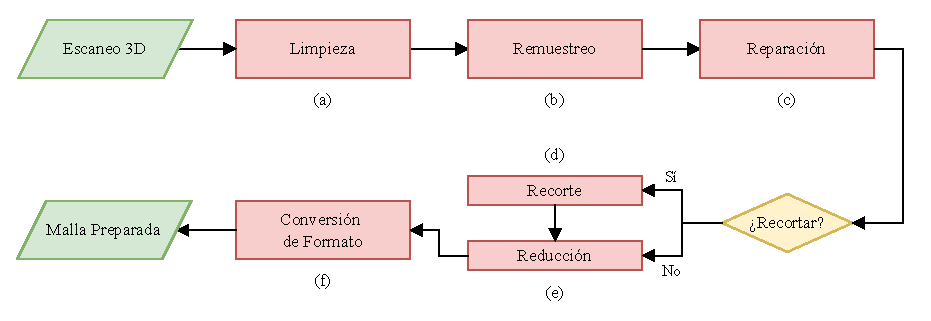
\includegraphics[width=\linewidth]{figures/4_materials-methods/mesh_preparation_pipeline.pdf}
    \caption[Diagrama resumen del preprocesado de datos]{Diagrama resumen del preprocesado de datos. Las mallas 3D escaneadas son primero limpiadas (a): se eliminan los materiales, geometría errónea y disconexa. Las mallas resultantes se remuestrean (b) para sellar los huecos existentes y obtener una geometría y topología uniforme. Este proceso puede reintroducir irregularidades, por lo que posteriormente se realiza una reparación adicional (c). A continuación, la malla puede recortarse (d) hasta un porcentaje de su tamaño original quitando partes no relevantes de la malla antes de ser simplificada (e) a un número determinado de triángulos. Finalmente, se convierten (f) al formato compatible con ExMeshCNN.}
    \label{mesh_preparation_pipeline}
\end{figure}

Como se ha mencionado en la Sección \ref{section4:materials}, los datos obtenidos para este proyecto provienen de escaneos de piezas anatómicas reales digitalizadas usando el escáner Artec Micro que permite captar datos en 3D en una zona de hasta 324 cm$^3$ y escanearlos con una precisión muy alta de hasta 10 micras y una resolución de hasta 0.029 mm \cite{artec_data}. Las mallas generadas a través de estos procesos resultan en geometrías incompletas, degeneradas y con gran variabilidad de resolución. Estos factores impiden su uso directo por el \textit{framework} de ExMeshCNN. Se tiene en la Figura \ref{mesh_preparation_pipeline} un diagrama que resume los pasos que se han tomado para preprocesar las mallas.

\subsubsection{Limpieza inicial de las mallas}
\begin{figure}[h]
    \centering
    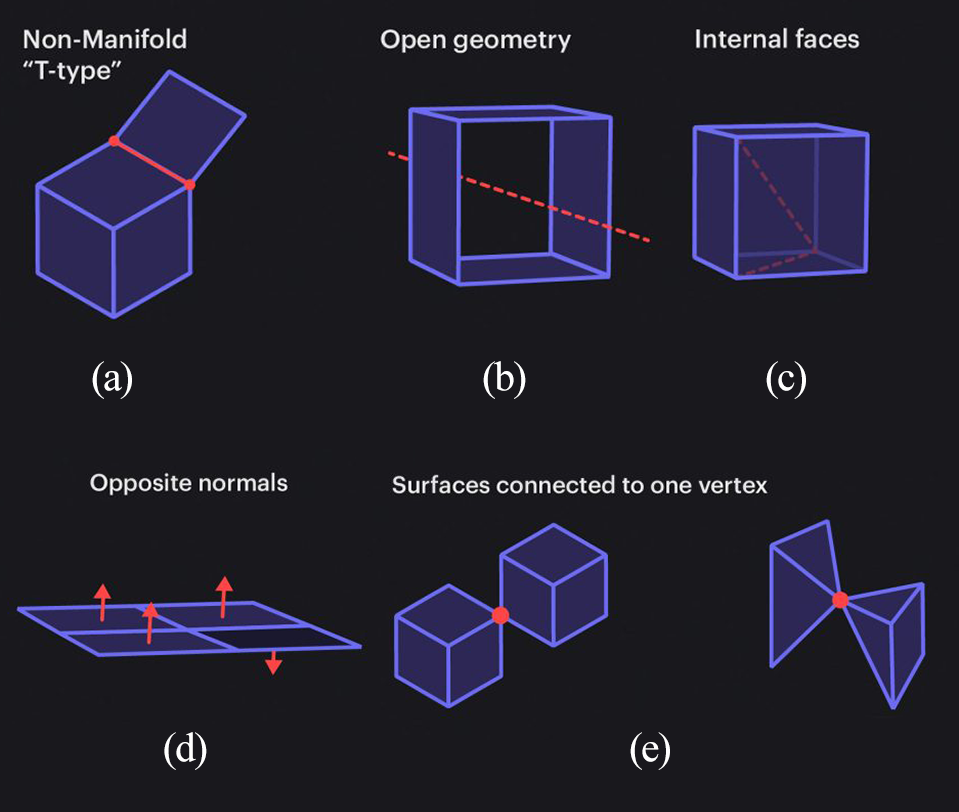
\includegraphics[width=0.8\linewidth]{figures/4_materials-methods/nonmanifold_examples.png}
    \caption[Ejemplo de mallas \textit{non-manifold}]{Ejemplo de mallas \textit{non-manifold}. Esto sucede cuando (a) existe una arista a la que se conectan tres caras, (b) la geometría no está sellada o no es \textit{watertight}, (c) se tienen caras dentro de partes selladas de la geometría, (d) hay normales invertidos y (e) cuando hay superficies conectadas solamente por un vértice. Figura adaptada de \cite{manifold_types_2021}.}
    \label{non_manifold_types}
\end{figure}

El primer paso del preprocesado consiste en la limpieza inicial de las mallas (paso (a) en la Figura \ref{mesh_preparation_pipeline}). En este paso, mediante un \textit{script} desarrollado con PyMeshLab, se busca eliminar la mayor cantidad posible de geometría no deseada presente en las mallas crudas obtenidas mediante escaneo 3D.

El proceso comienza eliminando las componentes desconectadas respecto a la componente principal; es decir, se eliminan fragmentos de geometría (ya sean triángulos o vértices) que no estén conectados a la porción principal de la malla así como vértices duplicados. A continuación, se realiza una primera limpieza para remover geometría degenerada (o de cero área) y parcialmente la geometría \textit{non-manifold}: aquella donde una arista se comparte por más de dos caras, alrededor de cada vértice, las caras no forman una vecindad contigua y hay bordes o agujeros. Para un ejemplo visual de este tipo de mallas, consultar la Figura \ref{non_manifold_types}. Realizado todo esto, se guarda una versión intermedia de la malla para su posterior procesamiento.

Para garantizar la consistencia de los datos y reducir posibles fuentes de ruido para el modelo, en el caso de las sínfisis púbicas derechas, se aplica un preprocesamiento adicional previo al paso de limpieza. Mediante un \textit{script} en Blender, se utiliza el modificador de espejo para reflejar estas mallas respecto al eje principal de simetría anatómica, transformándolas efectivamente en mallas equivalentes a las izquierdas.

\subsubsection{Remuestreo y sellado}
En este paso, las mallas intermedias se encuentran con una geometría y topología limpia exceptuando que las mallas no son \textit{watertight}: poseen huecos. Se tienen sellar necesariamente para su procesado por ExMeshCNN. El cierre de huecos en mallas 3D es una tarea compleja de realizar manualmente, pero puede abordarse de forma eficaz mediante una técnica alternativa: el remuestreo. Esta técnica genera una nueva topología manteniendo la forma superficial original de la malla. El proceso se basa en una aproximación iterativa mediante vóxeles, que reconstruye la superficie al tiempo que genera la conectividad necesaria para cerrar los huecos. Este paso corresponde al (b) de la Figura \ref{mesh_preparation_pipeline}.

Para ello, se empleó Blender, que dispone de un modificador de remuestreo robusto llamado \textit{Remesh}. Se desarrolló un segundo \textit{script} que toma como entrada la malla de salida del paso (a) y aplica el operador de remuestreo en modo \textit{SHARP}, con una profundidad del árbol octal de 10 (para preservar la fidelidad geométrica) y una escala de 1. El resultado es una malla libre de huecos, aunque este proceso puede reintroducir geometría \textit{non-manifold}.

La Figura \ref{remesh_hole_example} detalla el resultado de procesar la malla por este paso de preprocesado, obsérvese como el modificador sella por completo el hueco en la parte posterior de la malla 3D.

\begin{figure}[h]
    \centering
    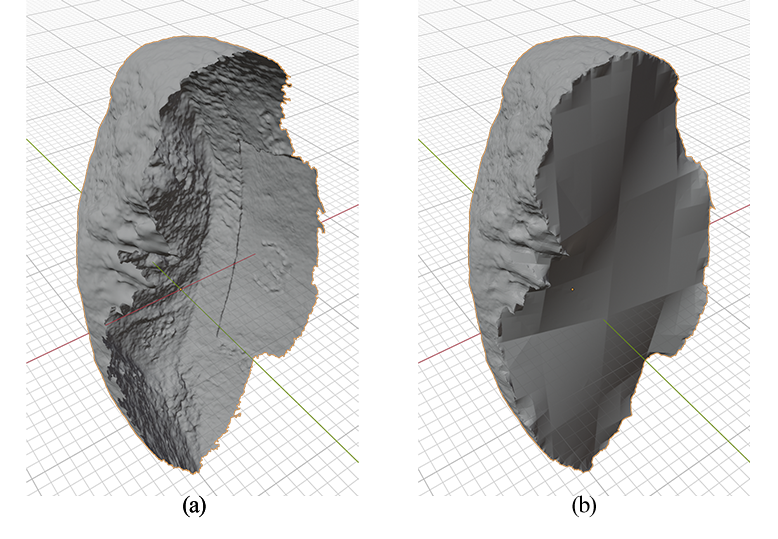
\includegraphics[width=\linewidth]{figures/4_materials-methods/remesh_hole_filled_example.png}
    \caption[Ejemplo de malla sellada por remuestreo]{Ejemplo de malla sellada mediante remuestreo. Se muestran las mallas vistas desde la parte posterior de la cara articular: en (a) se observa la malla tras el proceso de limpieza inicial, aún con un hueco visible en la zona posterior; en (b), la misma malla tras haber sido remuestrada durante el paso (b) del preprocesado (Figura \ref{mesh_preparation_pipeline}), donde dicho hueco ha sido sellado.}
    \label{remesh_hole_example}
\end{figure}

\subsubsection{Reparación de malla}
\label{section4:data_repair}
Debido a la posible reintroducción de geometría \textit{non-manifold} tras el remuestreo, se implementó en el mismo \textit{script} el paso (c) del preprocesado. Este paso consiste en un procedimiento iterativo diseñado para eliminar dicha geometría no válida. El procedimiento sigue los siguientes pasos:

\begin{enumerate}
    \item Se parte de la malla resultante del paso (b) (Figura \ref{mesh_preparation_pipeline}).
    \item Se seleccionan los vértices \textit{non-manifold} existentes. Si los hay, se realiza primero una eliminación de vértices duplicados, lo que en muchos casos deja la malla en un estado topológicamente válido.
    \item Se realiza una nueva selección de vértices \textit{non-manifold}. Si persisten, se colapsan vecindarios locales de dichos vértices en un único vértice con el fin de mitigar posibles huecos generados en pasos o iteraciones anteriores.
    \item Se repite la selección de vértices \textit{non-manifold}. Si aún existen, se eliminan directamente. Este paso puede generar nuevos huecos, que serán tratados en la siguiente iteración mediante el paso 3.
    \item Si persiste geometría \textit{non-manifold}, se retorna al paso 1; si la malla está reparada, el bucle finaliza.
\end{enumerate}

Se ha comprobado que, para los datos utilizados, este procedimiento converge tras un número finito de iteraciones, generando mallas completamente selladas y con una topología válida para su posterior procesamiento.

\subsubsection{Recorte de mallas}

\begin{figure}[htbp]
    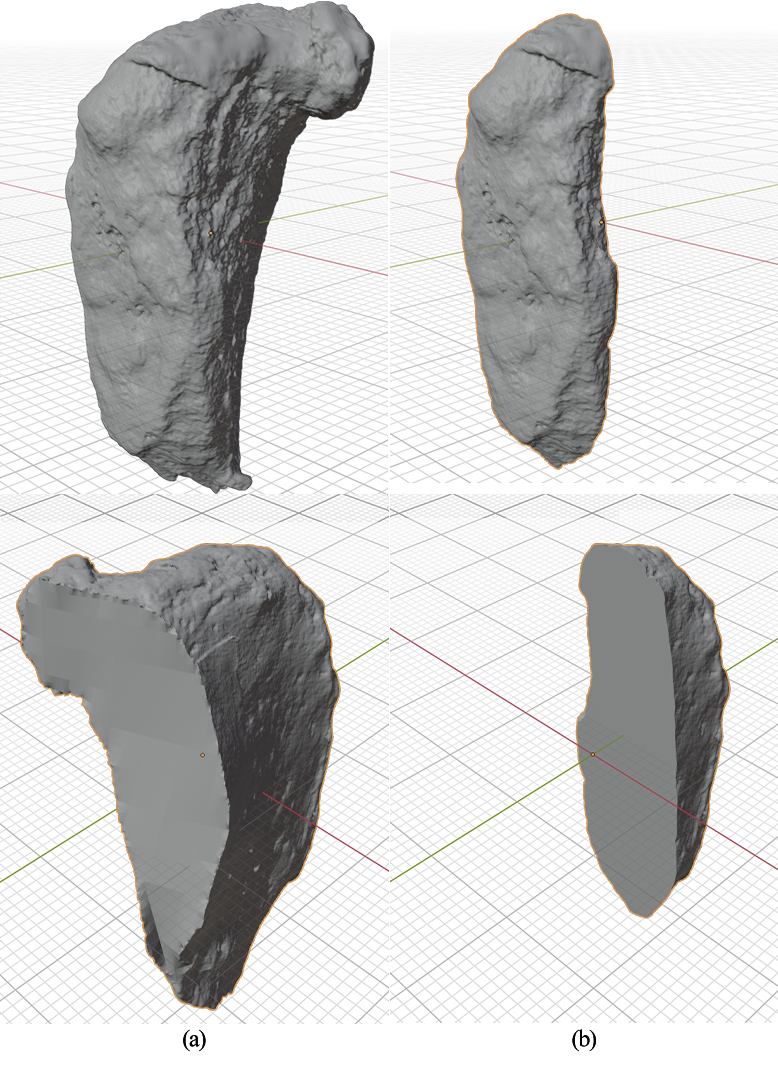
\includegraphics[width=\linewidth]{figures/4_materials-methods/bbox_cut_sample.png}
    \caption[Ejemplo de malla antes y después del recorte]{Ejemplo de malla antes y después del recorte. En (a) se observa la malla obtenida por el paso (c) vista de frente a la cara articular y por detrás de la misma. En (b) se observa la misma malla recortada, nótese la cantidad de geometría que se ha removido y que el recorte también genera mallas selladas.}
    \label{bbox_cut_sample}
\end{figure}

Obsérvese en la Figura \ref{mesh_preparation_pipeline} que existe una decisión entre los pasos (c) y (d) o (e) sobre recortar primero la malla antes de realizar la reducción de triángulos.

Se ha añadido este paso debido a que la reducción uniforme afecta por igual a todas las regiones de la malla, incluyendo zonas anatómicamente poco relevantes para el análisis forense, como la parte posterior y laterales del hueso respecto con la cara articular. Para maximizar la preservación de detalles en dicha cara articular siendo la región de interés, se implementó este proceso. Este consiste en realizar un recorte anatómico antes de la reducción de resolución, eliminando aquellas partes que los expertos forenses no consideran durante el análisis. Este doble enfoque permite disponer tanto de versiones completas como de versiones enfocadas en la cara articular, facilitando comparativas experimentales entre ambas modalidades de entrada.

El procedimiento, también automatizado mediante Blender, consiste en generar un cubo con las dimensiones de la malla (\textit{bounding box}) y reducirlo proporcionalmente para definir una región de interés. A continuación, se aplica un modificador booleano para recortar las partes externas no deseadas, lo cual es posible gracias a que todas las mallas están previamente alineadas en la misma orientación. Una vez realizado el recorte que también genera una malla sellada, se procede a aplicar la reducción de resolución. Se puede observar un ejemplo de una malla antes y después de haber sido recortada en la Figura \ref{bbox_cut_sample}.

\subsubsection{Reducción de resolución}
\label{section4:data_reduction}
Una vez obtenidas las mallas que presentan una geometría adecuada y sin defectos topológicos estando o no recortadas, persiste una variabilidad importante: el número de triángulos es diferente entre mallas. Para normalizar esta característica, se diseñó un \textit{script} que aplica una reducción global de resolución a la malla mediante colapso de aristas. Esto permite reducir de forma progresiva el número de triángulos, preservando en la medida de lo posible la topología general y los detalles relevantes. El resultado son mallas con un número fijo de triángulos especificado por el usuario. En el caso del proyecto actual se fijaron a valores de 100,000; 50,000 y 25,000 triángulos.

\subsubsection{Conversión de Formato}
Como último paso (f) del preprocesado, guiándose por la Figura \ref{mesh_preparation_pipeline}, se realiza la conversión de formato. Hasta este punto, las mallas han sido representadas mediante ficheros en formato OBJ. Sin embargo, ExMeshCNN, debido a los requisitos específicos que imponen sus descriptores y capas convolucionales, requiere que los datos estén en un formato particular utilizando el formato de guardado NPY de NumPy.

Esta conversión no altera la estructura de la malla, pero permite optimizar el proceso computacional. En lugar de procesar directamente los ficheros OBJ que implicaría un coste computacional adicional, la conversión permite calcular una única vez las características fijas de cada triángulo, que posteriormente serán utilizadas por los descriptores geométricos y geodésicos.

Una vez realizada esta transformación, las mallas en formato NPY están listas para ser utilizadas directamente por ExMeshCNN.

\FloatBarrier
\subsection{Búsqueda de Arquitectura Neuronal}
\label{section4:nas}
El procesamiento de mallas 3D mediante DL, como se ha comentado, constituye un campo aún en etapa experimental y en rápida evolución. Debido a su novedad, no existe un consenso establecido sobre cómo tratar estos datos de manera óptima. Como resultado, no se dispone de modelos preentrenados sobre mallas 3D con las características específicas requeridas en este trabajo, particularmente en el contexto de ExMeshCNN y con la resolución necesaria para abordar el presente problema.

Ante esta situación, se recurre a técnicas NAS, descritas con mayor profundidad en la Sección \ref{section2:nas}, con el fin de determinar tanto la estructura ideal así como los demás hiperparámetros de forma óptima de los modelos a emplear para el aprendizaje de las distintas características del método de Todd.

De entre las diversas herramientas disponibles para realizar NAS se ha seleccionado Optuna \cite{optuna_2019}, una biblioteca basada en optimización bayesiana que ha demostrado un alto rendimiento en tareas de generación automática de arquitecturas de red y ajuste de hiperparámetros \cite{pizurica_generic_2024}. Específicamente, se hace uso del algoritmo \textit{Tree-structured Parzen Estimator} (TPE), utilizado internamente por la biblioteca. 

Dado que las redes generadas en este proyecto presentan una complejidad relativamente baja en comparación con arquitecturas más generalistas, se optó por entrenarlas por completo y sin simplificar por 50 épocas, valor donde se observa que la mayoría de modelos convergen. Se aplica \textit{Model Checkpointing} para guardar automáticamente el modelo con mejor rendimiento alcanzado en la métrica F1 Macro del conjunto de validación. De este valor se deriva también la estimación de rendimiento de la arquitectura, es decir, la función objetivo que Optuna maximizará. Para más detalles sobre estas métricas, leer la Sección  \ref{section5:metrics}.

Los hiperparámetros considerados, junto con sus respectivos espacios de búsqueda, se detallan en la Tabla \ref{fig4:optuna_params} y la lógica detrás de la selección de estos se justifica del siguiente modo:

\begin{table}[h]
    \centering
    \begin{tabular}{|l|c|c|}
        \hline
        \rowcolor[HTML]{D33333} 
        {\color[HTML]{FFFFFF} \textbf{Hiperparámetro}} & {\color[HTML]{FFFFFF} \textbf{Valores posibles}} & {\color[HTML]{FFFFFF} \textbf{Tipo}} \\ \hline
        Tasa de Aprendizaje & $\left[1\times 10^{-5}, 1\times10^{-1}\right]$ & Rango \\ \hline
        Optimizador & \begin{tabular}[c]{@{}c@{}}Adam, AdamW, \\ Radam, SGD\end{tabular} & Categórica \\ \hline
        Inicialización de Pesos & \begin{tabular}[c]{@{}c@{}}Uniforme, Normal, \\ Xavier, Kaiming, \\ Ortogonal\end{tabular} & Categórica \\ \hline
        Escalado de Pesos & $\left[1, 10\right]$ & Rango \\ \hline
        Función de Pérdida & CE, WCE, FL, CBL & Categórica \\ \hline
        $\gamma$ de FL \textsuperscript{\textdagger} & $\left[1, 10\right]$ & Rango \\ \hline
        Tipo de CBL\textsuperscript{\textdaggerdbl} & Softmax, Sigmoide, FL & Categórica \\ \hline
        $\beta$ de CBL\textsuperscript{\textdaggerdbl} & $\left[0, 0.9999\right]$ & Rango \\ \hline
        \begin{tabular}[c]{@{}l@{}}Descriptor geodésico,\\ densidad de canal intermedio\end{tabular} & $\left[16, 32, 64, 128, 256\right]$ & Categórica \\ \hline
        \begin{tabular}[c]{@{}l@{}}Descriptor geodésico,\\ densidad de salida\end{tabular} & $\left[16, 32, 64, 128, 256\right]$ & Categórica \\ \hline
        \begin{tabular}[c]{@{}l@{}}Descriptor geométrico,\\ densidad de canal intermedio\end{tabular} & $\left[16, 32, 64, 128, 256\right]$ & Categórica \\ \hline
        \begin{tabular}[c]{@{}l@{}}Descriptor geométrico,\\ densidad de salida\end{tabular} & $\left[16, 32, 64, 128, 256\right]$ & Categórica \\ \hline
        Nº de capas convolucionales & $\left[2, 6\right]$ & Rango \\ \hline
        \begin{tabular}[c]{@{}l@{}}Densidad capa \\ convolucional $i$-ésima\end{tabular} & $\left[16, 32, 64, 128, 256\right]$ & Categórica \\ \hline
        Nº de capas densas & $\left[1, 5\right]$ & Rango \\ \hline
        Densidad capa densa $i$-ésima & $\left[8, 16, 32, 64, 128, 256\right]$ & Categórica \\ \hline
    \end{tabular}
    \caption[Hiperparámetros utilizados por Optuna]{Hiperparámetros utilizados en el entrenamiento con Optuna junto a su espacio de búsqueda. El tipo \say{rango} indica que cualquier valor entre los indicados puede ser utilizado, mientras que el tipo \say{categórico} indica que solamente se pueden emplear los valores listados. Funciones de pérdida: CE: \textit{Cross-Entropy}; WCE: \textit{Weighted Cross-Entropy}; FL: \textit{Focal Loss}; CBL: \textit{Class-Balanced Loss}. \textbf{\textdagger}: Solo se aplica si la función de pérdida seleccionada es FL. \textbf{\textdaggerdbl}: Solo se aplica si la función de pérdida seleccionada es CBL.}
    \label{fig4:optuna_params}
\end{table}


\begin{itemize}
    \item \textbf{Optimizadores:} Se consideran variantes ampliamente utilizadas de la familia Adam, incluyendo AdamW y RAdam, que han demostrado mejoras empíricas sobre el algoritmo original en diversos contextos. Asimismo, se incluye el algoritmo clásico de Descenso de Gradiente Estocástico (SGD), dado que en ciertos escenarios puede superar el rendimiento de Adam, especialmente en términos de generalización.
    \item \textbf{Tasa de aprendizaje:} El rango seleccionado corresponde al intervalo recomendado en la literatura para los optimizadores considerados. Optuna se encarga de explorar combinaciones y descartar automáticamente aquellas que conduzcan a un rendimiento subóptimo. 
    \item \textbf{Inicialización y escalado de pesos:} Estos parámetros se incluyen debido a su impacto potencial sobre la estabilidad y eficiencia del entrenamiento. Se ha demostrado que en ciertos problemas, la elección adecuada de inicialización puede marcar una diferencia significativa en la calidad del aprendizaje.
    \item \textbf{Funciones de pérdida:} Dado el fuerte desbalance presente en las etiquetas, se han incorporado varias funciones diseñadas específicamente para tratar este tipo de problemas. Además de la función clásica de entropía cruzada (CE), se incluyen su versión ponderada (\textit{Weighted Cross-Entropy}, WCE), la pérdida Focal (FL), y la pérdida Class-Balanced (CBL), cada una con ventajas particulares para abordar clases minoritarias. Para una descripción detallada de estas funciones, véase la Sección \ref{section5:metrics}.
    \item \textbf{Parámetros específicos de funciones de pérdida:} Cuando la función de pérdida seleccionada es FL o CBL, se incluyen los hiperparámetros adicionales requeridos, cuyos valores se han establecido siguiendo las recomendaciones de los autores de dichas técnicas.
    \item \textbf{Arquitectura de red:} Dado que los descriptores también constituyen capas con parámetros entrenables, se ha considerado su densidad (relación entre tamaño de entrada y salida) como un hiperparámetro a explorar, utilizando valores típicos en capas convolucionales. En cuanto al número total de capas, se optó por arquitecturas compactas, priorizando capas convolucionales sobre totalmente conectadas, con el objetivo de maximizar la eficiencia computacional y la capacidad expresiva dentro de los límites de memoria de las GPUs utilizadas. Debido a que las capas convolucionales de ExMeshCNN incluyen ya \textit{Batch Normalization} internamente no se consideró añadir más regularización al modelo en cuanto a arquitectura.
    \item \textbf{Densidades de capas:} Los valores posibles para la densidad de capas se han tomado de configuraciones comúnmente utilizadas en redes profundas, procurando siempre que las configuraciones más grandes posibles puedan ajustarse dentro de la memoria disponible del hardware.
\end{itemize}

Cabe destacar que, para los experimentos multietiqueta, se han tomado decisiones específicas respecto a los hiperparámetros y la arquitectura de los modelos:

\begin{itemize}
    \item Las funciones de pérdida se asignan de manera independiente por Optuna a cada una de las características incluidas en el experimento. Esto permite optimizar el comportamiento del modelo respecto a cada etiqueta específica, ajustando la función objetivo según la naturaleza de cada característica.
    
    \item La estructura de la red en los experimentos multietiqueta difiere de la utilizada en los experimentos de etiqueta única. En particular, la parte totalmente conectada de la red se ramifica en tantas salidas como características se estén prediciendo, esta decisión se basa en \cite{ranjan_hyperface_2019}, donde se utilizó esta misma metodología satisfactoriamente. Las ramificaciones puede adoptar dos configuraciones distintas: una en la que todas las subredes comparten la misma arquitectura (en términos de número de capas y densidad de neuronas), y otra en la que cada subred posee una arquitectura completamente independiente del resto. Esto permite obtener la mayor variedad de arquitecturas posibles, con la esperanza de obtener modelos con el mejor rendimiento posible para cada característica. La parte convolucional de la red se mantiene idéntica para cualquiera de los casos.
\end{itemize}

Dicho todo esto, todas las arquitecturas generadas por NAS siguen una estructura base predefinida, que actúa como un \say{esqueleto} arquitectónico. Esta estructura consta de tres bloques principales dispuestos secuencialmente: (1) un bloque de entrada conformado por los descriptores geométricos y geodésicos, (2) un bloque convolucional compuesto por varias capas 1D convolucionales, y (3) un bloque totalmente conectado (denso), precedido por una capa de \textit{pooling} que conecta ambas partes. El proceso de búsqueda se encarga de optimizar aspectos internos de cada bloque (número de capas, tamaño de filtros, densidad de neuronas, etc.), pero mantiene inalterada esta macroestructura. Se puede observar un ejemplo de esta macroestructura en la Figura \ref{nas_macrostruct} tanto para modelos que usan una única etiqueta como para aquellos que usan múltiples.

\begin{figure}[h]
    \begin{subfigure}{\textwidth}
        \centering
        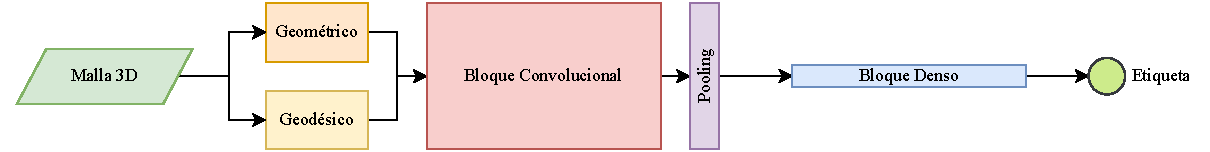
\includegraphics[width=\linewidth]{figures/4_materials-methods/NAS_sample1.pdf}
        \caption{Macroestructura de red para modelos de etiqueta única.}
        \label{single_label_nets}
    \end{subfigure}

    \begin{subfigure}{\textwidth}
        \centering
        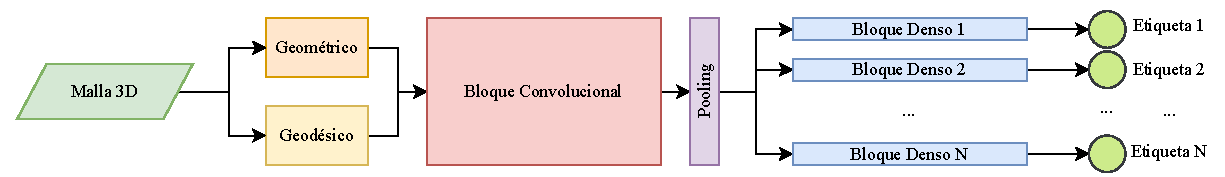
\includegraphics[width=\linewidth]{figures/4_materials-methods/NAS_sample2.pdf}
        \caption{Macroestructura de red para modelos multietiqueta.}
        \label{multi_label_nets}
    \end{subfigure}
    \caption[Macroestructura de redes generadas por NAS]{Macroestructura de redes generadas por NAS. Todas las redes poseen esta arquitectura genérica: una malla 3D se procesará primero por las capas de descriptores, luego pasará por el bloque convolucional llegando hasta el bloque denso por medio de una capa de \textit{pooling} como nexo. En (a) se muestra la macroestructura de los modelos de etiqueta única, en (b) la de los modelos multietiqueta, obsérvese que las ramificaciones en estos modelos son solamente de los bloques de capas densas.}
    \label{nas_macrostruct}
\end{figure}


\section{Protocolo de validación experimental}
Para el entrenamiento de los modelos se empleó la técnica de \textit{hold-out}, que consiste en dividir el conjunto de datos en dos subconjuntos principales: uno de entrenamiento y otro de test. A su vez, el conjunto de entrenamiento se subdivide para obtener un subconjunto adicional de validación. Durante el proceso de entrenamiento, el modelo es ajustado utilizando únicamente los datos del conjunto de entrenamiento, mientras que el conjunto de validación se utiliza para monitorizar el rendimiento del modelo en cada época, permitiendo detectar fenómenos como el sobreajuste para finalizar el entrenamiento aplicando \textit{Early Stopping}, almacenar el mejor modelo por medio del \textit{Model Checkpointing} y orientar el ajuste de hiperparámetros. Una vez completado el entrenamiento, el modelo final se evalúa utilizando el conjunto de test, que se ha mantenido completamente aislado durante todo el proceso de ajuste, proporcionando así una estimación objetiva del rendimiento general del modelo sobre datos no vistos. Se optó por esta estrategia en lugar de una validación cruzada tradicional de $n$ particiones ($n$-fold cross-validation), debido al elevado coste computacional que implicaría. Aunque la arquitectura ExMeshCNN presenta una buena eficiencia, el uso conjunto con técnicas de NAS multiplica considerablemente el tiempo necesario para cada experimento, haciendo que aplicar $n$-fold CV resulte intratable en los plazos estimados para este proyecto.

Como se describió en la Sección \ref{section4:data_preparation}, se utilizan tanto huesos izquierdos como derechos de los individuos. Dado que, desde el punto de vista anatómico, ambos presentan una alta similitud morfológica, realizar la partición del conjunto de datos a nivel de muestra podría provocar una fuga de información (\textit{data leakage}). Para evitar este problema, la división se llevó a cabo a nivel de individuo: todos los huesos pertenecientes a un mismo sujeto se incluyen exclusivamente en uno de los subconjuntos (entrenamiento, validación o test), sin solapamiento entre ellos. Esto garantiza que el modelo no memorice rasgos individuales específicos, sino que generalice adecuadamente aprendiendo patrones morfológicos relevantes.

Uno de los retos más significativos de este trabajo es el marcado desbalance entre clases presente en los datos, una condición que afecta directamente la capacidad del modelo para generalizar adecuadamente. Este desbalance varía entre las diferentes características del método de Todd, y en muchos casos existen clases con muy pocos ejemplos en comparación con otras (véase Sección \ref{section4:data_eda} para más detalles), dificultando el aprendizaje robusto y equitativo. Debido a ello, no resulta viable utilizar una única partición común para todas las características, ya que esto podría conducir a una representación muy deficiente de ciertas clases en algunas tareas, afectando negativamente el rendimiento del modelo. Por esta razón, se optó por realizar una división estratificada individual para cada característica, maximizando así su representación interna y permitiendo un proceso de entrenamiento más efectivo. No se han podido aplicar técnicas de \textit{undersampling} debido a la ya limitada cantidad de datos disponibles, ni técnicas de \textit{oversampling}, ya que no existen actualmente métodos capaces de generar nuevos ejemplos sintéticos que preserven de manera realista la geometría y morfología de las mallas óseas. Además, transformaciones geométricas clásicas como rotaciones, escalados uniformes o traslaciones no son consideradas como instancias nuevas dentro del \textit{framework}, al tratarse de modificaciones que no alteran la relación entre los vecindarios de triángulos de las mallas.

En los experimentos multietiqueta, donde varias características se modelan simultáneamente, el problema del desbalance se intensifica, ya que se debe considerar la combinación de distribuciones entre etiquetas. Para mitigar este efecto, se utilizó una técnica de estratificación iterativa \cite{sechidis2011stratification, pmlr-v74-szymański17a}, que permite preservar de forma aproximada la distribución conjunta de etiquetas en los subconjuntos generados. Esto reduce significativamente la pérdida de información estructural entre clases y ayuda a mantener un equilibrio relativo, mitigando en parte las dificultades impuestas por el fuerte desbalance, uno de los principales desafíos técnicos del proyecto. 

En todos los experimentos se aplicó la misma proporción en la división de los datos, siguiendo la recomendación habitual para la técnica \textit{hold-out}: se empleó un 65\% del total para el conjunto de entrenamiento, un 15\% para validación y el 20\% restante para test.

\section{Funciones de pérdida y métricas de rendimiento}
\label{section5:metrics}
Dado que se trata de un problema de clasificación, se emplea la función de pérdida de entropía cruzada (\textit{cross-entropy loss}) para ajustar los pesos y sesgos de las neuronas del modelo. Esta función se define de la siguiente forma:

\begin{equation}
L_{CE} = -\sum_i^n t_i \log(p_i)
\end{equation}

Donde $n$ es el número de clases, $t_i$ es la etiqueta verdadera (1 si la clase es la correcta, 0 en caso contrario) y $p_i$ es la probabilidad predicha para la $i$-ésima clase. Esta función penaliza con mayor intensidad aquellas predicciones que se alejan de la clase verdadera, incentivando al modelo a asignar una alta probabilidad a la clase correcta. Cuando la predicción es certera, el valor de la función tiende a cero; en cambio, si el modelo asigna baja probabilidad a la clase correcta, la función tiende a valores grandes positivos.

Adicionalmente, dado que el problema presenta un desbalance de clases, se han incorporado funciones de pérdida específicamente diseñadas para afrontar esta problemática. En particular, se han utilizado: la versión ponderada de la entropía cruzada (\textit{Weighted Cross Entropy}, WCE), la pérdida Focal (FL) y la pérdida Class-Balanced (CBL).

\begin{align}
    L_{WCE} &= -\sum_i^n \alpha_{i} t_i \log(p_i) \\
    L_{FL} &= -\sum_i^n (1-p_i)^{\gamma} t_i \log(p_i) \\
    L_{CB}(\textbf{p},y) &= \frac{1-\beta}{1-\beta^{n_{y}}} \mathcal{L}(\textbf{p},y)
\end{align}

En la WCE, el término $\alpha_i$ representa un peso específico para cada clase $i$, utilizado para reescalar la contribución de cada término de la pérdida. En este trabajo, se ha calculado $\alpha_i$ como el inverso de la frecuencia de la clase correspondiente, de modo que las clases menos representadas obtienen mayor peso, contrarrestando el sesgo del modelo hacia las clases mayoritarias.

Por su parte, la pérdida Focal (FL) \cite{lin_focal_2020} extiende este enfoque mediante la incorporación del término $(1 - p_i)^\gamma$, donde $\gamma$ es un parámetro ajustable denominado factor de enfoque. Esta formulación reduce el impacto de las muestras correctamente clasificadas, es decir, aquellas con alta probabilidad en la clase verdadera y amplifica el efecto de aquellas muestras más difíciles de clasificar. Al hacerlo, se logra que el modelo se concentre en los casos menos representados.

La pérdida Class-Balanced (CBL) \cite{cui_class-balanced_2019}, en cambio, introduce una formulación más refinada del peso por clase, basada en el número efectivo de muestras. En lugar de utilizar directamente la frecuencia inversa de las clases, CBL calcula un factor de corrección con el parámetro $\beta$ que refleja mejor la cantidad de información aportada por cada clase. Esta técnica puede aplicarse como un prefactor sobre diferentes funciones de pérdida $\mathcal{L}(\mathbf{p}, y)$, siendo compatible tanto con WCE como con FL, entre otras.

Aunque estas funciones de pérdida son fundamentales para guiar el proceso de entrenamiento y seleccionar el mejor modelo, no ofrecen información directa sobre el rendimiento del clasificador en términos de aciertos y errores. Para ello, se emplea la métrica de exactidud o \textit{accuracy}, que cuantifica la proporción de muestras clasificadas correctamente. Esta métrica se define como:

\begin{equation}
\text{Accuracy} = \frac{TP + TN}{TP + TN + FP + FN}
\end{equation}

donde $TP$ (verdaderos positivos) y $TN$ (verdaderos negativos) representan las predicciones correctas, mientras que $FP$ (falsos positivos) y $FN$ (falsos negativos) corresponden a errores de clasificación.

A pesar de su carácter intuitivo y simplicidad, el \textit{accuracy} puede inducir a interpretaciones erróneas cuando se trabaja con conjuntos de datos desbalanceados, ya que no distingue entre los distintos tipos de errores y puede sobreestimar el rendimiento del modelo en clases mayoritarias.

Por ello, se incluye la métrica F1, que representa un balance armónico entre \textit{precision} y \textit{recall}:
\begin{equation}
    \text{F1} = 2 \cdot \frac{\text{Precision} \cdot \text{Recall}}{\text{Precision} + \text{Recall}}
\end{equation}

donde las métricas de \textit{precision} y \textit{recall}, en el contexto binario, se definen como:
\begin{align}
    \text{Precision} &= \frac{TP}{TP + FP} \\
    \text{Recall} &= \frac{TP}{TP + FN}
\end{align}

La \textit{precision} indica qué proporción de las predicciones positivas realizadas por el modelo son correctas, mientras que \textit{recall} mide la proporción de muestras realmente positivas que fueron correctamente identificadas. Estas métricas permiten detectar posibles sesgos en el comportamiento del modelo, tales como una mayor propensión a cometer falsos positivos o falsos negativos.

Dado que en este proyecto se persigue una clasificación lo más equilibrada posible entre clases, se adopta como métrica principal la media macro del F1 (F1 Macro). Esta variante calcula primero el F1 de cada clase de forma individual y luego promedia estos valores, asignando el mismo peso a todas las clases sin considerar su frecuencia en el conjunto de datos. Esta propiedad la hace especialmente adecuada para contextos con fuerte desbalance de clases, como es el caso de este trabajo, ya que penaliza con mayor severidad los errores cometidos en las clases minoritarias. En consecuencia, el F1 Macro se emplea como criterio principal para evaluar y comparar el rendimiento de los modelos entrenados. Su formulación matemática es la siguiente:
\begin{align}
    \text{F1}_{\text{Macro}} &=  2 \cdot \frac{\text{Precision}_{\text{Macro}} \cdot \text{Recall}_{\text{Macro}}}{\text{Precision}_{\text{Macro}} + \text{Recall}_{\text{Macro}}} 
\end{align}
Dado que su cálculo se basa en las versiones multiclase de \textit{precision} y \textit{recall}, estas se definen como:
\begin{align}
    \text{Precision}_{\text{Macro}} &= \frac{\text{Precision}_{\text{Clase A}}+\text{Precision}_{\text{Clase B}}+\dots+\text{Precision}_{\text{Clase N}}}{N} \\
    \text{Recall}_{\text{Macro}} &= \frac{\text{Recall}_{\text{Clase A}}+\text{Recall}_{\text{Clase B}}+\dots+\text{Recall}_{\text{Clase N}}}{N}
\end{align}

Durante el proceso de NAS, como se detalla en la Sección \ref{section4:nas}, fue necesario definir una función objetivo (\textit{fitness}) que guiara la optimización. Dada la naturaleza desbalanceada del problema, se eligió la métrica F1 Macro como base para esta función. El valor de fitness se define como:
\begin{equation}
    \text{Fitness} = \text{F1}_{\text{Macro}_{\text{Validación}}} \cdot (1 - | \text{F1}_{\text{Macro}_{\text{Validación}}} -  \text{F1}_{\text{Macro}_{\text{Entrenamiento}}}|)
\end{equation}

La heurística de esta formulación es la siguiente: por un lado, se favorecen modelos con un alto rendimiento en el conjunto de validación, y por otro, se penaliza la discrepancia entre el rendimiento en entrenamiento y validación, lo cual es indicativo de sobreajuste. De este modo, se priorizan aquellos modelos que generalizan bien y no simplemente memorizan los datos de entrenamiento. De esta forma también se logra mitigar el desbalance de los datos en el aprendizaje de los modelos.

\section{Experimentos}
Con el conjunto de datos ya preprocesado y las configuraciones del \textit{framework} ExMeshCNN definidas, en esta sección se describen los experimentos llevados a cabo para evaluar la viabilidad y el rendimiento del enfoque propuesto. El objetivo principal es analizar la capacidad de diferentes modelos para predecir automáticamente las características morfológicas del método de Todd a partir de mallas 3D de la sínfisis del pubis, considerando tanto esquemas de clasificación individual como multietiqueta.

En primer lugar, en la Subsección \ref{section5:experiment_edge_collapse}, se analiza cuantitativamente la pérdida de fidelidad geométrica resultante de reducir el número de triángulos en las mallas. Esta operación es necesaria para garantizar una resolución uniforme entre todas las muestras y, al mismo tiempo, hacer posible el entrenamiento de los modelos con los recursos computacionales disponibles. Por tanto, este análisis permite justificar el uso de versiones simplificadas de las mallas en el resto de experimentos.

A continuación, en la Subsección \ref{unique_tag_exps}, se presentan los experimentos de clasificación por etiqueta única, en los cuales se entrena un modelo independiente para cada una de las nueve características del método de Todd. Se describen las configuraciones utilizadas, se analizan los resultados obtenidos y se discute el rendimiento de los mejores modelos para cada etiqueta.

Luego, en la Subsección \ref{multi_tag_exps}, se exponen los experimentos de clasificación multietiqueta. En este caso, se entrenan modelos capaces de predecir simultáneamente múltiples características, ya sea utilizando las nueve características completas o subconjuntos de características altamente asociadas entre sí. Se evalúa su rendimiento y se comparan los resultados con los obtenidos en los experimentos de etiqueta única.

En la Subsección \ref{best_models_analysis}, se presenta un estudio detallado de los mejores modelos obtenidos para las nueve características, sean de etiqueta única o múltiple. Se analizan en mayor detalle su aprendizaje por medio de sus respectivas matrices de confusión, con el fin de interpretar más finamente sus capacidades discriminativas.

Finalmente, en la Subsección \ref{gradcam_analysis}, se presenta una visualización de las regiones de activación generadas mediante Grad-CAM, aplicada a las predicciones de los mejores modelos entrenados. El objetivo es identificar las zonas morfológicas que cada modelo considera relevantes para clasificar las distintas características del método de Todd. Se analiza si dichas regiones varían entre características, así como su consistencia a lo largo de diferentes muestras. Este análisis busca proporcionar evidencia adicional de que los modelos han aprendido a generalizar de forma coherente los datos y la existencia de zonas diferenciadas de interés para cada característica.

\subsection{Análisis de pérdida de calidad de mallas 3D al reducir el número de triángulos}
\label{section5:experiment_edge_collapse}
Como se ha explicado en la Sección \ref{section4:methods}, el método ExMeshCNN requiere que todas las mallas tengan un número idéntico de caras triangulares para poder procesarlas correctamente. Sin embargo, como se mencionó en la Sección \ref{section4:data_preparation}, las mallas del conjunto de datos original presentan un número variable de triángulos, y además, muchas de ellas contienen una cantidad excesiva de caras que supera las capacidades del hardware disponible.

Por este motivo, es importante evaluar el impacto que tiene la reducción del número de triángulos sobre la calidad topológica de las mallas. En particular, se busca responder la siguiente pregunta: ¿en qué medida se ve afectada la topología de una malla al aplicar técnicas de simplificación por colapso de aristas?

\begin{figure}[h]
    \centering
    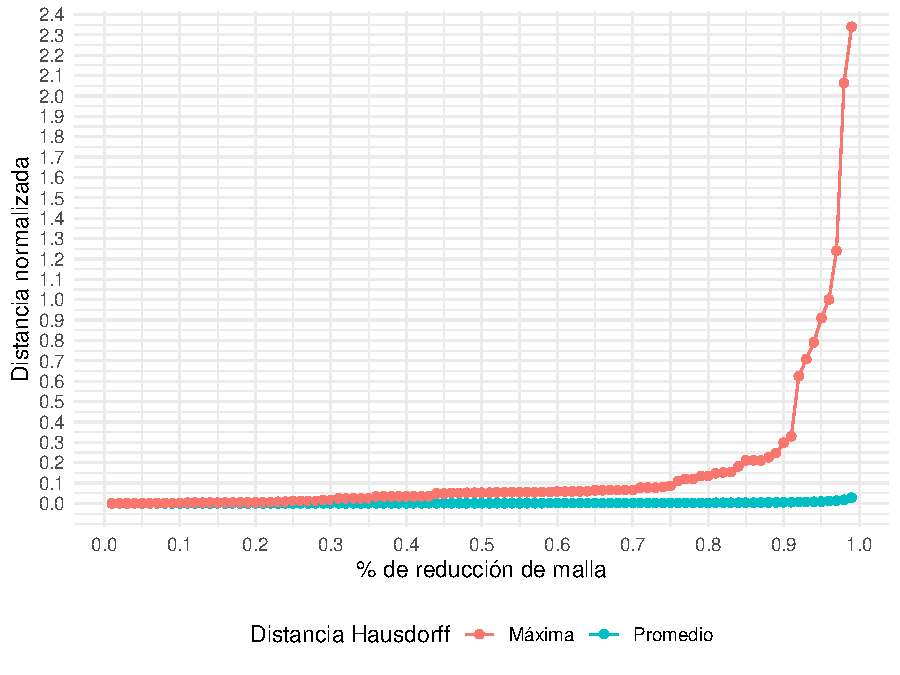
\includegraphics[width=\linewidth]{figures/5_experiments/mesh_redux_study.pdf}
    \caption[Estudio de reducción de mallas]{Distancia Hausdorff normalizada por \textit{bounding box} entre las mallas originales y sus versiones reducidas a distintos porcentajes del número original de triángulos. En este experimento, la reducción se realizó en incrementos del 1\%. Se observa la media del error de todos los triángulos y el valor máximo entre dos triángulos de la malla original y la reducida. Nótese que el error medio se mantiene bastante bajo, mientras que el máximo empieza a dispararse al sobrepasar el 90\% de reducción del tamaño original.}
    \label{fig5:redux_study}
\end{figure}

Para abordar esta cuestión, se diseñó un experimento en el que se tomaron diez mallas aleatoriamente del conjunto de datos original y se generaron versiones reducidas conservando distintas proporciones del número de triángulos originales (por ejemplo, 75\%, 50\%, 25\%, etc.). Posteriormente, estas versiones simplificadas se comparan con la malla original utilizando la distancia de Hausdorff, con el fin de cuantificar la desviación de la superficie resultante respecto de la original. Formalmente, esta distancia se define como:

\begin{equation}
d_H = \max\left\{\sup_{x\in X} \inf_{y \in Y} d(x,y), \sup_{y\in Y} \inf_{x \in X} d(x,y) \right\}
\end{equation}

donde $X$ e $Y$ son subconjuntos del espacio métrico, y $d(x,y)$ representa la distancia entre los puntos $x$ e $y$. En el contexto de las mallas 3D \cite{cignoni1998metro}, se evalúa esta métrica entre triángulos de dos mallas distintas, permitiendo cuantificar la similitud o diferencia entre sus superficies.

En la Figura \ref{fig5:redux_study} se presenta la evolución de la distancia Hausdorff normalizada al reducir progresivamente el número de triángulos de las mallas con el error medio de la malla y el error máximo obtenido entre dos triángulos de la misma. Esta distancia ha sido normalizada respecto a la diagonal de la \textit{bounding box} de cada malla original, lo que permite comparar directamente las deformaciones relativas entre mallas de diferentes tamaños y complejidades geométricas, además facilita el cálculo de promedios globales entre las distintas muestras evaluadas. Esto se puede interpretar también como un porcentaje de error, o de variación entre las mallas originales y reducidas.

Como puede observarse, hasta una reducción del 75\% del número de triángulos, el error promedio permanece esencialmente cercano a cero, lo que sugiere una alta fidelidad en la preservación de la geometría original. Durante este mismo rango, el error máximo crece lentamente, manteniéndose inferior al 2\% de variación con respecto a la malla original. Es únicamente a partir de reducciones superiores al 90\% cuando se observa un incremento más pronunciado y exponencial del error máximo, aunque el error promedio aún se mantiene bastante bajo.

Estos resultados apuntan a que es posible aplicar reducciones agresivas en la cantidad de triángulos sin comprometer significativamente la calidad topológica de las mallas. En consecuencia, se valida la viabilidad de utilizar versiones simplificadas de las mallas para el entrenamiento mediante ExMeshCNN. A partir de esta observación, se decide emplear tres niveles de resolución: 100,000, 50,000 y 25,000 triángulos.

El valor de 100,000 triángulos se establece como umbral máximo, ya que permite entrenar los modelos en un tiempo razonable con los recursos computacionales disponibles. Además, el análisis mediante la distancia de Hausdorff demuestra que incluso con una reducción del 90\% respecto a la media de triángulos de las mallas originales, la superficie resultante conserva de media una geometría suficientemente cercana a la original. Por otro lado, las resoluciones de 50,000 y 25,000 triángulos se incluyen con el fin de evaluar cómo afecta una reducción más drástica en la calidad de los resultados. Esto es motivado por los autores de ExMeshCNN, que sugieren que el \textit{framework} obtiene un mejor rendimiento con resoluciones más bajas.

\subsection{Experimentos con etiqueta única}
\label{unique_tag_exps}
Una vez validado que es factible utilizar versiones reducidas de las mallas sin pérdida significativa de información, y habiendo preparado los datos para su uso con el modelo ExMeshCNN, tal como se describe en la Sección \ref{section4:data_preparation}, se procedió a diseñar la estrategia de NAS, explicada en profundidad en la Sección \ref{section4:nas}.

En esta fase, se llevaron a cabo los denominados experimentos de etiqueta única, donde se entrena un modelo independiente para cada una de las características de Todd, sin considerar la influencia de las demás características. Por cada característica, se realizaron 6 ejecuciones distintas resultantes de las combinaciones de los siguientes parámetros:

\begin{itemize}
\item \textbf{Resolución de la malla}: 100,000 (abreviado a 100K); 50,000 (50K) o 25,000 (25K) triángulos.
\item \textbf{Tipo de malla}: Malla completa (abreviado a \textit{Full}) o malla recortada (\textit{Cut}), ver Figura \ref{bbox_cut_sample}.
\end{itemize}

Tomando en cuenta que la estrategia de NAS emplea 50 épocas por cada entrenamiento, cada ejecución del proceso implica la realización de 200 entrenamientos distintos para encontrar la arquitectura más adecuada para predecir cada característica de forma individual. Este valor se seleccionó como un compromiso entre la necesidad de una exploración suficientemente amplia del espacio de búsqueda del NAS y las limitaciones prácticas impuestas por el tiempo de cómputo del hardware disponible. Dado que se trabajó con las 9 características del método de Todd, y que para cada una se evaluaron 6 combinaciones diferentes de configuración, el número total de entrenamientos realizados asciende a $9 \times 6 \times 200 =$ 10,800. Esto representa 1,800 entrenamientos por característica, reflejando el elevado grado de exhaustividad y robustez aplicado para asegurar modelos óptimos y bien ajustados en cada caso.

El tiempo requerido por cada ejecución varió en función de la resolución de la malla utilizada independientemente del tipo de malla, así como de la complejidad de las arquitecturas evaluadas por Optuna en cada uno de los 200 entrenamientos. A pesar de esta variabilidad, se observó que: las ejecuciones con mallas de 100K triángulos requerían entre 7 y 8 días completos; las de 50K triángulos, entre 3 y 4 días; y las de 25K triángulos, alrededor de 1 a 2 días por ejecución.

\begin{table}[h]
    \centering
    \begin{tabular}{|c|c|c|c|c|}
    \hline
    \rowcolor[HTML]{D33333} 
    {\color[HTML]{FFFFFF} \textbf{Característica}} & {\color[HTML]{FFFFFF} \textbf{Test Acc}} & {\color[HTML]{FFFFFF} \textbf{Test F1}} & {\color[HTML]{FFFFFF} \textbf{Resolución}} & {\color[HTML]{FFFFFF} \textbf{Tipo}} \\ \hline
    AF & 0.65 & 0.47 & 50K & \textit{Cut} \\
    BN & 0.92 & 0.69 & 25K & \textit{Cut} \\
    DM & 0.73 & 0.63 & 25K & \textit{Cut} \\
    DP & 0.88 & 0.71 & 25K & \textit{Cut} \\
    IP & 0.71 & 0.54 & 100K & \textit{Cut} \\
    LSE & 0.98 & 0.92 & 100K & \textit{Full} \\
    USE & 0.98 & 0.83 & 25K & \textit{Cut} \\
    VB & 0.52 & 0.53 & 50K & \textit{Cut} \\
    VM & 0.70 & 0.67 & 50K & \textit{Cut} \\ \hline
    \end{tabular}
    \caption[Cuadro resumen de los mejores modelos obtenidos para cada característica]{Cuadro resumen de los mejores modelos obtenidos para cada característica en el conjunto de datos de test. Las columnas \say{Test Acc} y \say{Test F1} indican los valores obtenidos para las métricas de \textit{accuracy} y F1 Macro respectivamente. La columna \say{Tipo} indica si se ha utilizado la malla completa (\textit{Full}) o la versión recortada (\textit{Cut}), véase Figura \ref{bbox_cut_sample}.}
    \label{table5:single_tag__results}
\end{table}

Como se puede observar en la Tabla \ref{table5:single_tag__results}, existe una considerable variabilidad en los valores obtenidos para la métrica F1 Macro al evaluar cada modelo sobre el conjunto de test. No obstante, en la mayoría de los casos se han alcanzado resultados satisfactorios, con valores de F1 Macro superiores a 0.5 en todos los modelos menos uno (en el que se alcanza más de 0.47), además de un \textit{accuracy} generalmente elevado (igual o superior a 0.7 en siete características).

Es particularmente destacable el desempeño de las características LSE y USE, que han alcanzado resultados sobresalientes a pesar de presentar un alto grado de desbalance en las etiquetas, como se evidenció en el EDA (Sección \ref{section4:data_eda}). Esto sugiere la presencia de patrones bien definidos en la superficie ósea que han sido correctamente capturados por los modelos, permitiendo lograr simultáneamente un \textit{accuracy} muy alto y valores de F1 Macro igualmente notables. En contraste, otras dos características también altamente desbalanceadas, como BN y DP, si bien obtuvieron buenos resultados, se encuentran dentro del rango de desempeño general de las demás características más balanceadas, lo que refuerza la hipótesis de que LSE y USE presentan una topología más informativa o distinguible para las redes.

Por otro lado, la característica VB, que presenta la distribución más balanceada de etiquetas, fue la que obtuvo el rendimiento más bajo tanto en términos de \textit{accuracy} como de F1 Macro. Esto podría indicar que, pese a un buen balance, los patrones topológicos asociados a esta característica son más sutiles o complejos de identificar, lo cual plantea un reto adicional para el modelo.

El resto de las características muestran un comportamiento relativamente uniforme, sin una clara correlación entre el grado de desbalance y el rendimiento del modelo, lo que a su vez sugiere que el enfoque de entrenamiento adoptado ha sido eficaz para extraer información relevante incluso en escenarios con clases altamente desbalanceadas y una cantidad limitada de datos.

Un aspecto adicional a destacar es el impacto del tipo de malla utilizada. Exceptuando el modelo de LSE, todos los demás alcanzaron mejores resultados al emplear las versiones recortadas de las mallas. Este comportamiento respalda la hipótesis de que eliminar estructuras óseas irrelevantes (según la práctica de los expertos) permite concentrar el poder de representación del modelo en la zona de interés, reduciendo el ruido y facilitando la identificación de patrones significativos. En el caso de LSE, sin embargo, las mallas completas resultaron más beneficiosas, lo cual podría implicar que la información relevante para esta característica se encuentra distribuida también fuera de la región de la cara articular de la sínfisis.

Respecto a la resolución, se observa que los mejores resultados, en general, se obtuvieron con la resolución más baja de 25K triángulos, seguida de 50K, y solo dos modelos alcanzaron su mejor desempeño con 100K triángulos. Esta observación concuerda con lo reportado por los autores de ExMeshCNN \cite{kim_exmeshcnn_2022}, donde también se encontró que las mallas de menor resolución producían mejores resultados. Esto se puede deber a que, al aumentar la resolución, la operación de \textit{global average pooling} que conecta las capas convolucionales con las totalmente conectadas podría estar diluyendo información crítica al comprimir un mayor número de triángulos en una única representación.

Sin embargo, las características LSE e IP constituyen una excepción a esta tendencia: en ambos casos, la mayor resolución permitió obtener un mejor rendimiento, lo que indica que para estas características el mayor nivel de detalle en la superficie ósea proporciona una ventaja en el aprendizaje del modelo.

\subsection{Experimentos multietiqueta}
\label{multi_tag_exps}
Una vez realizados los experimentos de etiqueta única, se procedió a entrenar modelos capaces de predecir múltiples características simultáneamente. Para ello, se empleó el enfoque de \textit{multi-label classification}, que permite que cada muestra del conjunto de datos pueda estar asociada a más de una etiqueta, en contraste con la clasificación tradicional donde cada muestra pertenece a una única clase. 

Cabe destacar que, si bien los modelos entrenados en estos experimentos son efectivamente multietiqueta, el objetivo último no es necesariamente obtener un único modelo capaz de predecir de forma óptima todas las características simultáneamente. Más bien, se busca evaluar si el aprendizaje conjunto de varias características puede mejorar el rendimiento en la predicción individual de cada una. Por ello, incluso si un modelo multietiqueta logra un rendimiento significativamente superior en una única característica, aunque su rendimiento en otras no sea destacable, dicho modelo es de interés para esa característica específica. Esto permite valorar modelos multietiqueta no como soluciones integrales, sino también como posibles especializaciones con beneficios colaterales derivados del aprendizaje compartido.

Siguiendo esta lógica, primero se realizaron 200 entrenamientos con todas las características de Todd por cada resolución, tipo de malla y, adicionalmente, dos configuraciones de la parte densa o totalmente conectada del modelo: una donde todas las salidas poseen la misma estructura (abreviado a \textit{Same}) y otra donde cada salida tiene una estructura densa independiente (\textit{Variable}). Nuevamente se utilizan 200 épocas para mantener la consistencia y por la misma razón que en el experimento de etiqueta única. Es decir $2 \times 2 \times 3 \times 200 = 2,400$ entrenamientos.

Posteriormente, se llevaron a cabo ejecuciones adicionales utilizando la mejor combinación de resolución de malla y tipo de malla obtenidos para cada característica individual en los experimentos de etiqueta única, junto con las tres características que presentan mayor asociación con ella, según los valores de la T de Tschuprow mostrados en la Tabla \ref{table4:corr}. En este caso, también se evaluaron ambas configuraciones de la parte densa del modelo (\textit{Same} y \textit{Variable}), utilizando igualmente 200 épocas. O sea, $9 \times 2 \times 200 = 3,600$ entrenamientos con las tres características con mayor asociación a una característica dada.

El tiempo requerido varió no solo en función de la resolución de las mallas, sino que también se vio influido por la complejidad de la parte densa del modelo. Como era de esperar, los modelos con mayor número de características y resolución elevada fueron los que presentaron mayores requerimientos computacionales: Para las configuraciones con nueve características y resolución de 100K triángulos, el tiempo de entrenamiento se situó entre 28 y 30 días continuos. Con 50K triángulos, la duración se redujo a aproximadamente 15 días, y con 25K triángulos, a unos 7 días.

En los experimentos con cuatro características, los tiempos se redujeron considerablemente: Con mallas de 100K triángulos, los entrenamientos tomaron alrededor de 10 días; con 50K triángulos, cerca de 5 días y con 25K triángulos, aproximadamente 3 o 4 días por ejecución. Estos tiempos evidencian el alto coste computacional del proceso experimental, así como el compromiso asumido para lograr una validación exhaustiva de los modelos generados.

\begin{table}[h]
    \centering
    \resizebox{\textwidth}{!}{%
    \begin{tabular}{|cc|c|c|c|c|c|}
        \hline
        \rowcolor[HTML]{D33333} 
        \multicolumn{2}{|c|}{\cellcolor[HTML]{D33333}{\color[HTML]{FFFFFF} \textbf{Característica}}} & \cellcolor[HTML]{D33333}{\color[HTML]{FFFFFF} } & \cellcolor[HTML]{D33333}{\color[HTML]{FFFFFF} } & \cellcolor[HTML]{D33333}{\color[HTML]{FFFFFF} } & \cellcolor[HTML]{D33333}{\color[HTML]{FFFFFF} } & \cellcolor[HTML]{D33333}{\color[HTML]{FFFFFF} } \\ \cline{1-2}
        \rowcolor[HTML]{D33333} 
        \multicolumn{1}{|c|}{\cellcolor[HTML]{D33333}{\color[HTML]{FFFFFF} \textbf{Evaluada}}} & {\color[HTML]{FFFFFF} \textbf{Soporte}} & \multirow{-2}{*}{\cellcolor[HTML]{D33333}{\color[HTML]{FFFFFF} \textbf{\begin{tabular}[c]{@{}c@{}}Test \\ Acc\end{tabular}}}} & \multirow{-2}{*}{\cellcolor[HTML]{D33333}{\color[HTML]{FFFFFF} \textbf{\begin{tabular}[c]{@{}c@{}}Test \\ F1\end{tabular}}}} & \multirow{-2}{*}{\cellcolor[HTML]{D33333}{\color[HTML]{FFFFFF} \textbf{Resolución}}} & \multirow{-2}{*}{\cellcolor[HTML]{D33333}{\color[HTML]{FFFFFF} \textbf{Tipo}}} & \multirow{-2}{*}{\cellcolor[HTML]{D33333}{\color[HTML]{FFFFFF} \textbf{Estructura Densa}}} \\ \hline
        \multicolumn{1}{|c|}{AF} & DM, LSE, USE & 0.69 & 0.52 & 50K & \textit{Cut} & \textit{Variable} \\
        \multicolumn{1}{|c|}{BN} & AF, DP, LSE & 0.91 & 0.79 & 25K & \textit{Cut} & \textit{Variable} \\
        \multicolumn{1}{|c|}{DM} & Todas & 0.80 & 0.65 & 100K & \textit{Cut} & \textit{Same} \\
        \multicolumn{1}{|c|}{DP} & Todas & 0.93 & 0.72 & 100K & \textit{Cut} & \textit{Same} \\
        \multicolumn{1}{|c|}{IP} & Todas & 0.67 & 0.48 & 50K & \textit{Full} & \textit{Same} \\
        \multicolumn{1}{|c|}{LSE} & DM, USE, VM & 0.95 & 0.79 & 100K & \textit{Full} & \textit{Variable} \\
        \multicolumn{1}{|c|}{USE} & AF, DM, LSE & 0.95 & 0.86 & 25K & \textit{Cut} & \textit{Same} \\
        \multicolumn{1}{|c|}{VB} & Todas & 0.49 & 0.48 & 50K & \textit{Cut} & \textit{Same} \\
        \multicolumn{1}{|c|}{VM} & AF, DM, IP & 0.70 & 0.50 & 100K & \textit{Cut} & \textit{Variable} \\ \hline
    \end{tabular}%
    }
    \caption[Resultados de los mejores modelos obtenidos para cada característica en los experimentos multietiqueta]{Resultados de los mejores modelos obtenidos para cada característica en los experimentos multietiqueta en el conjunto de datos de test. Las columnas \say{Test Acc} y \say{Test F1} indican los valores obtenidos para las métricas de \textit{accuracy} y F1 Macro respectivamente. La columna \say{Tipo} indica si se ha utilizado la malla completa (\textit{Full}) o la versión recortada (\textit{Cut}), véase Figura \ref{bbox_cut_sample}. La columna \say{Estructura Densa} indica si el modelo utiliza la misma estructura densa para las salidas de la red (\textit{Same}) o si cada salida puede variar independiente del resto (\textit{Variable}), véase Subsección \ref{section4:nas}.}
    \label{table5:multilabel_results}
    \end{table}

De estos 6000 entrenamientos, en la Tabla \ref{table5:multilabel_results} se muestran los resultados de los mejores modelos obtenidos para cada característica. Se observa que existe más variedad respecto a la resolución de las mallas empleadas. Sorpresivamente, se encuentran casi de forma equitativa las resoluciones de 25K, 50K y 100K triángulos, con 4 modelos utilizando 100K, 3 modelos con 50K y 2 modelos con 25K. Esto contrasta con los experimentos de etiqueta única, donde la mayoría de los modelos se entrenaron con mallas de 25K triángulos. Esto resulta interesante porque sugiere que, al entrenar modelos multietiqueta, la información contenida en las mallas de mayor resolución puede ser más relevante para la predicción de múltiples características simultáneamente y no se ve tan diluida como pasa tanto con entrenamientos de etiqueta única, como los realizados anteriormente o los realizados por los autores de ExMeshCNN.

Por parte de los tipos de malla, esto se ha mantenido constante respecto a los experimentos de etiqueta única, ya que la mayoría de los modelos se entrenaron con mallas recortadas (\textit{Cut}), excepto en el caso de las características LSE e IP, que emplearon mallas completas (\textit{Full}). Esto refuerza la idea de que, para ciertas características (en el caso de etiqueta única, LSE, y ahora tanto LSE como IP), la información contenida en las zonas no recortadas es crucial para lograr un buen rendimiento del modelo incluso en un contexto multietiqueta.

En cuanto a la estructura de las capas totalmente conectadas, se observa que no hay una preferencia clara entre las distintas configuraciones, estando distribuidas casi equitativamente, esto sugiere que la elección de la estructura densa puede depender más de la naturaleza específica de las características a predecir que de una tendencia generalizada.

Sobre las características de soporte, nuevamente se encuentra una distribución casi equitativa entre hacer uso de todas las características o las tres con mayor asociación con la característica de interés. Esto indica que, al entrenar modelos multietiqueta, es beneficioso considerar un conjunto amplio de características para mejorar la capacidad predictiva del modelo, no existiendo una tendencia clara hacia un enfoque u otro, al menos en estos experimentos.

\begin{table}[h]
    \centering
    \begin{tabular}{|c|cc|cc|}
        \hline
        \rowcolor[HTML]{D33333} 
        \cellcolor[HTML]{D33333}{\color[HTML]{FFFFFF} } & \multicolumn{2}{c|}{\cellcolor[HTML]{D33333}{\color[HTML]{FFFFFF} \textbf{Etiqueta Única}}} & \multicolumn{2}{c|}{\cellcolor[HTML]{D33333}{\color[HTML]{FFFFFF} \textbf{Etiqueta Múltiple}}} \\ \cline{2-5} 
        \rowcolor[HTML]{D33333} 
        \multirow{-2}{*}{\cellcolor[HTML]{D33333}{\color[HTML]{FFFFFF} \textbf{Característica}}} & \multicolumn{1}{c|}{\cellcolor[HTML]{D33333}{\color[HTML]{FFFFFF} \textbf{Test Acc}}} & {\color[HTML]{FFFFFF} \textbf{Test F1}} & \multicolumn{1}{c|}{\cellcolor[HTML]{D33333}{\color[HTML]{FFFFFF} \textbf{Test Acc}}} & {\color[HTML]{FFFFFF} \textbf{Test F1}} \\ \hline
        AF & \multicolumn{1}{c|}{0.65} & 0.47 & \multicolumn{1}{c|}{0.69} & \textbf{0.52} \\
        BN & \multicolumn{1}{c|}{0.92} & 0.69 & \multicolumn{1}{c|}{0.91} & \textbf{0.79} \\
        DM & \multicolumn{1}{c|}{0.73} & 0.63 & \multicolumn{1}{c|}{0.80} & \textbf{0.65} \\
        DP & \multicolumn{1}{c|}{0.88} & 0.71 & \multicolumn{1}{c|}{0.93} & \textbf{0.72} \\
        IP & \multicolumn{1}{c|}{0.71} & \textbf{0.54} & \multicolumn{1}{c|}{0.67} & 0.48 \\
        LSE & \multicolumn{1}{c|}{0.98} & \textbf{0.92} & \multicolumn{1}{c|}{0.95} & 0.79 \\
        USE & \multicolumn{1}{c|}{0.98} & 0.83 & \multicolumn{1}{c|}{0.95} & \textbf{0.86} \\
        VB & \multicolumn{1}{c|}{0.52} & \textbf{0.53} & \multicolumn{1}{c|}{0.49} & 0.48 \\
        VM & \multicolumn{1}{c|}{0.70} & \textbf{0.67} & \multicolumn{1}{c|}{0.70} & 0.50 \\ \hline
    \end{tabular}
    \caption[Comparación de resultados entre los mejores modelos obtenidos en los experimentos de etiqueta única y multietiqueta]{Comparación de resultados entre los mejores modelos obtenidos en los experimentos de etiqueta única y multietiqueta en el conjunto de datos de test. Se observan en las columnas \say{Test Acc} y \say{Test F1} los valores obtenidos para las métricas de \textit{accuracy} y F1 Macro respectivamente. Los valores en negrita indican los mejores resultados obtenidos de la métrica F1 Macro para cada característica.}
    \label{table5:multilabel_comparison}
\end{table}

Finalmente, se observa que los resultados obtenidos en los experimentos multietiqueta poseen una ligera ventaja sobre los de etiqueta única, observándose la Tabla \ref{table5:multilabel_comparison}, donde 5 de las 9 características mejoran la métrica F1 Macro respecto a sus contrapartes de etiqueta única. Esto sugiere que el modelo es capaz de aprender patrones más complejos y representativos al considerar múltiples características simultáneamente, lo que a su vez puede mejorar la generalización del modelo y su capacidad para capturar relaciones entre las distintas características. Siendo esto consistente con la literatura consultada, donde se ha demostrado que los modelos multietiqueta pueden beneficiarse de la correlación o asociación entre las etiquetas para mejorar el rendimiento general del modelo \cite{ranjan_hyperface_2019}. Si bien existe más disparidad respecto al \textit{accuracy} entre los experimentos de etiqueta única y multietiqueta, en general se observa que se mantiene un rendimiento alto en ambas configuraciones, con valores muy similares a los obtenidos en los experimentos de etiqueta única.

\subsection{Análisis de los mejores modelos}
\label{best_models_analysis}
Durante los experimentos realizados, se ha observado que los modelos son capaces de aprender patrones topológicos relevantes en las mallas óseas para predecir las características de Todd. Los resultados obtenidos tanto en los experimentos de etiqueta única como en los de multietiqueta muestran un rendimiento prometedor, con valores de \textit{accuracy} y F1 Macro que evidencian una buena capacidad de generalización por parte de los modelos, lo que a su vez demuestra una buena selección tanto de espacio de búsqueda como de estrategia de búsqueda de la técnica de NAS empleada. Esto también deja en evidencia la efectividad del \textit{framework} de ExMeshCNN en datos reales.

\begin{figure}[htbp]
    \centering
    \begin{subfigure}[t]{0.3\textwidth}
        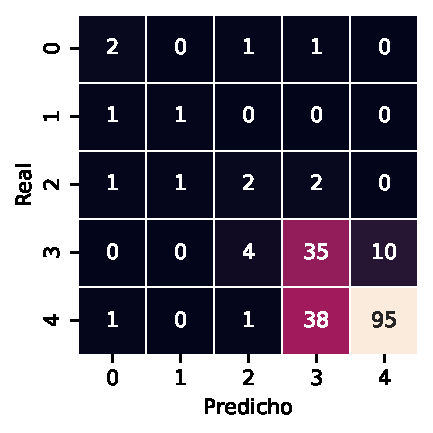
\includegraphics[width=\textwidth]{figures/5_experiments/multi-af-cm.pdf}
        \caption{\textbf{AF}: \textit{Acc} = 0.69; F1 = 0.52. Leyenda: \textbf{0}: Porosidad Regular, \textbf{1}: Muy Definidas, \textbf{2}: Poco Profundas, \textbf{3}: Restos de Surcos, \textbf{4}: No hay surcos.}
        \label{fig5:AF_confusion_matrix}
    \end{subfigure} 
    \begin{subfigure}[t]{0.3\textwidth}
        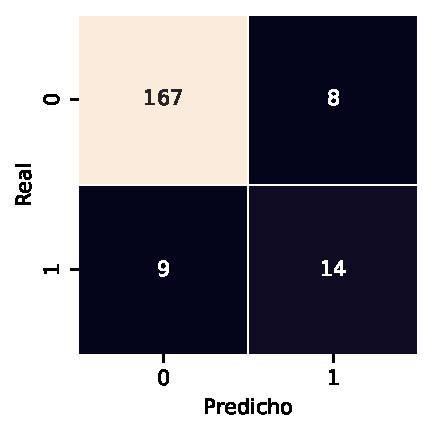
\includegraphics[width=\textwidth]{figures/5_experiments/multi-bn-cm.pdf}
        \caption{\textbf{BN}: \textit{Acc} = 0.91; F1 = 0.79. Leyenda: \textbf{0}: Ausente, \textbf{1}: Presente.}
        \label{fig5:BN_confusion_matrix}
    \end{subfigure} 
    \begin{subfigure}[t]{0.3\textwidth}
        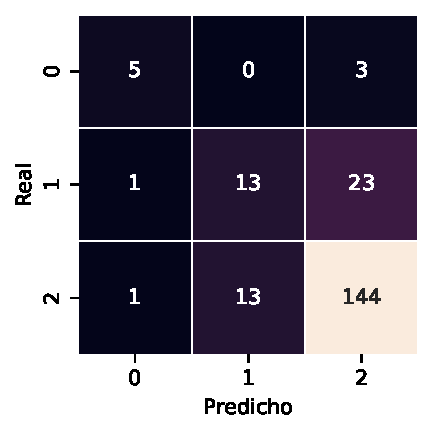
\includegraphics[width=\textwidth]{figures/5_experiments/multi-dm-cm.pdf}
        \caption{\textbf{DM}: \textit{Acc} = 0.80; F1 = 0.65. Leyenda: \textbf{0}: No Definido, \textbf{1}: En Formación, \textbf{2}: Definido.}
        \label{fig5:DM_confusion_matrix}
    \end{subfigure}
    \begin{subfigure}[t]{0.3\textwidth}
        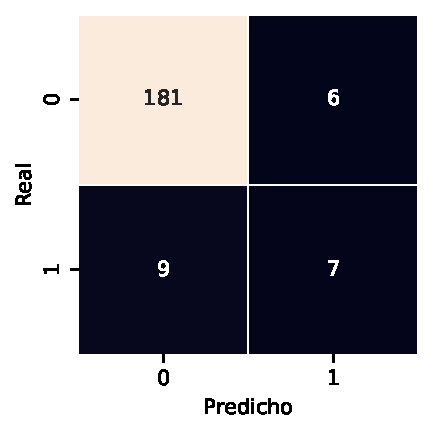
\includegraphics[width=\textwidth]{figures/5_experiments/multi-dp-cm.pdf}
        \caption{\textbf{DP}: \textit{Acc} = 0.93; F1 = 0.72. Leyenda: \textbf{0}: Ausente, \textbf{1}: Presente.}
        \label{fig5:DP_confusion_matrix}
    \end{subfigure}  
    \begin{subfigure}[t]{0.3\textwidth}
        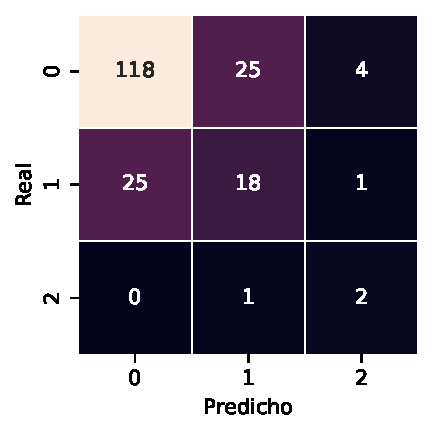
\includegraphics[width=\textwidth]{figures/5_experiments/single-ip-cm.pdf}
        \caption{\textbf{IP}: \textit{Acc} = 0.71; F1 =  0.54. Leyenda: \textbf{0}: No, \textbf{1}: Mediana, \textbf{2}: Sí.}
        \label{fig5:IP_confusion_matrix}

    \end{subfigure}  
    \begin{subfigure}[t]{0.3\textwidth}
        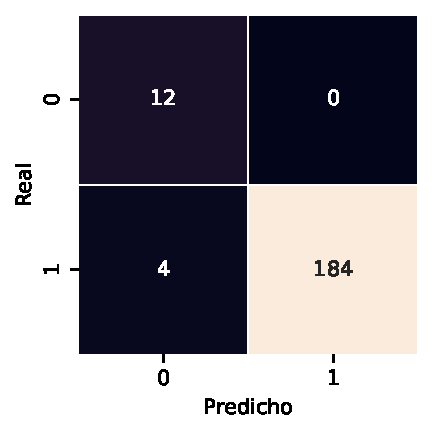
\includegraphics[width=\textwidth]{figures/5_experiments/single-lse-cm.pdf}
        \caption{\textbf{LSE}: \textit{Acc} = 0.98; F1 = 0.92. Leyenda: \textbf{0}: No Definido, \textbf{1}: Definido.}
        \label{fig5:LSE_confusion_matrix}
    \end{subfigure}  
    \begin{subfigure}[t]{0.3\textwidth}
        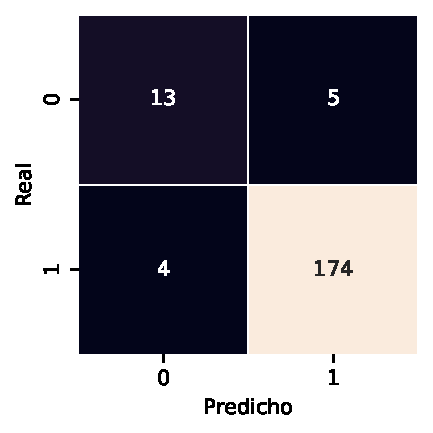
\includegraphics[width=\textwidth]{figures/5_experiments/multi-use-cm.pdf}
        \caption{\textbf{USE}: \textit{Acc} = 0.95; F1 = 0.86. Leyenda: \textbf{0}: No Definido, \textbf{1}: Definido.}
        \label{fig5:USE_confusion_matrix}
    \end{subfigure}
    \begin{subfigure}[t]{0.3\textwidth}
        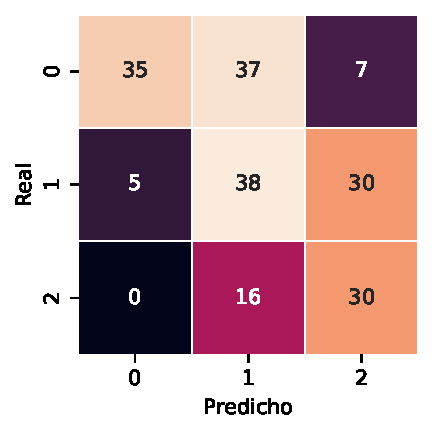
\includegraphics[width=\textwidth]{figures/5_experiments/single-vb-cm.pdf}
        \caption{\textbf{VB}: \textit{Acc} = 0.52; F1 = 0.53. Leyenda: \textbf{0}: Ausente, \textbf{1}: En Formación, \textbf{2}: Presente.}
        \label{fig5:VB_confusion_matrix}
    \end{subfigure}  
    \begin{subfigure}[t]{0.3\textwidth}
        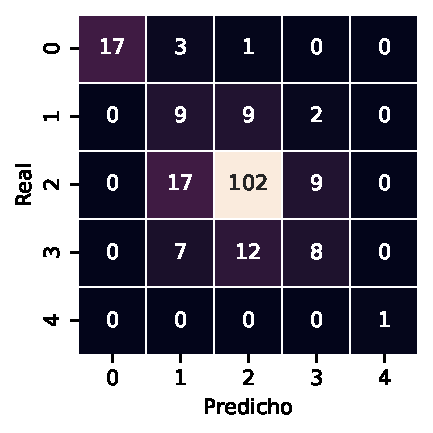
\includegraphics[width=\textwidth]{figures/5_experiments/single-vm-cm.pdf}
        \caption{\textbf{VM}: \textit{Acc} = 0.70; F1 = 0.67. Leyenda: \textbf{0}: Ausente, \textbf{1}: En Formación, \textbf{2}: Formado, Sin Excrecencias, \textbf{3}: Formado, Pocas Excrecencias, \textbf{4}: Formado, Muchas Excrecencias.}
        \label{fig5:VM_confusion_matrix}
    \end{subfigure}  
    \caption[Matrices de confusión de los mejores modelos en datos de test]{Matrices de confusión de los mejores modelos por cada característica en datos de test. Los valores de \say{\textit{Acc}} y \say{F1} indican el \textit{accuracy} y F1 Macro respectivamente.}
    \label{conf_matrices}
\end{figure}


Al analizar las matrices de confusión de los mejores modelos para cada característica en la Figura \ref{conf_matrices}, se observa que los modelos tienden a clasificar correctamente la mayoría de las muestras de forma equilibrada, cometiendo más errores en aquellas clases menos representadas. Este comportamiento es coherente con lo esperado en problemas de clasificación desbalanceada, donde los modelos suelen favorecer las clases mayoritarias. No obstante, la mayoría de las confusiones ocurren entre clases adyacentes, lo que sugiere que el modelo ha aprendido a capturar patrones estructurales relevantes en las características de Todd, incluso si los límites entre clases no son del todo nítidos. Además, el análisis de las matrices de confusión revela que la calidad real de los modelos es superior a la que podría inferirse exclusivamente a partir de la métrica F1 Macro. Esto resulta razonable, dado que dicha métrica es particularmente conservadora y fue seleccionada deliberadamente para ejercer una presión adicional durante la optimización, favoreciendo modelos que mantuvieran un buen rendimiento incluso en clases minoritarias.

Respecto a las características, como se ha evidenciado en los experimentos, la más fácil de predecir es LSE (Subfigura \ref{fig5:LSE_confusion_matrix}), seguida de cerca por USE (Subfigura \ref{fig5:USE_confusion_matrix}). Resulta notable que este comportamiento también se refleja en la percepción de los humanos: según Irurita et al. \cite{irurita2025pubic}, estas dos características son las menos complejas de identificar, tanto para expertos forenses como para principiantes, en base a los errores intra- e inter-observador. Asimismo, se confirma que la característica VB representa la mayor dificultad, coincidiendo con los resultados experimentales: VB obtuvo el \textit{accuracy} más bajo y el segundo valor más bajo de F1 Macro. Esta convergencia entre modelos y juicio experto aporta credibilidad tanto a los resultados obtenidos como a la validez del método de Todd.

Sin embargo, también se evidencian ciertas discrepancias. Por ejemplo, el artículo señala que la característica AF es relativamente sencilla de identificar para los forenses, algo que no se refleja en los experimentos: AF presenta el segundo peor \textit{accuracy} y el peor F1 Macro de todas las características. Esta divergencia podría deberse a una menor cantidad de datos disponibles para esta característica o a una falta de expresividad en el modelo, que le impide captar los patrones que los humanos sí logran identificar. Por otro lado, las características BN y DP muestran un rendimiento elevado en los experimentos, mientras que en el estudio antropológico presentan un grado de error considerable, especialmente en las evaluaciones realizadas por forenses novatos. 

Los mejores modelos obtenidos presentan arquitecturas notablemente diversas, reflejando la eficacia del proceso de NAS para adaptarse a los requisitos de cada característica. Aun así, se observa una tendencia general hacia redes con mayor profundidad convolucional y estructuras tipo cuello de botella, especialmente en características complejas como AF, BN o VM. También destacan patrones recurrentes como el uso del optimizador Adam, la inicialización Kaiming y funciones de pérdida adaptadas al desbalance de clases, como WCE y CBL. Si bien algunos hiperparámetros muestran comportamientos consistentes, otros, como el \textit{learning rate} o las capas totalmente conectadas, varían según la tarea. Para una descripción más detallada consultar el Anexo \ref{best_model_arch}, donde también se pueden observar las arquitecturas obtenidas para cada uno de los nueve mejores modelos.


\subsection{Visualización de áreas de interés con Grad-CAM}
\label{gradcam_analysis}

Se empleó el método Grad-CAM para visualizar las regiones de las mallas en las que se enfocan los modelos al realizar sus predicciones. En la Figura \ref{fig5:grad_cam__diff_chars} se muestra un ejemplo comparativo entre distintas características, donde puede observarse que cada modelo se centra en una zona distinta de la sínfisis del pubis. Esto refuerza la idea de que los modelos han aprendido patrones morfológicos específicos para cada característica, localizados en distintas áreas del hueso. 

Adicionalmente, se presentan ejemplos individuales de activación de Grad-CAM en las Figuras \ref{fig5:grad_cam__BN_samples}, \ref{fig5:grad_cam__USE_samples} y \ref{fig5:grad_cam__DP_samples}, correspondientes a las características BN, USE y DP, respectivamente. En estos casos, se observa que las zonas de atención se mantienen relativamente consistentes entre distintas muestras, aunque con variaciones según la etiqueta.

En particular, para la característica BN, el modelo concentra su atención en la parte superior de la sínfisis del pubis. Para USE, las activaciones se localizan principalmente en la parte superior izquierda del hueso, con extensiones hacia los laterales y zonas planas de la superficie. Finalmente, para DP, el modelo se enfoca de forma bastante localizada en un solo lateral del hueso. Naturalmente, existen otras características cuyas áreas de interés no se encuentran tan bien definidas, también es necesario tomar en cuenta que es posible que Grad-CAM se vea afectado por el hecho de haber utilizado clasificación multietiqueta, puesto que las gradientes de las otras características puedan interferir con el área de interés de la característica que se está analizando.

En todo caso estos resultados dan buenos indicios sobre la validez de los modelos entrenados tomando en cuenta el resto del análisis y aportan evidencia de que las características morfológicas definidas por el método de Todd pueden ser localizadas objetivamente en la superficie del hueso mediante técnicas de DL. Esto representa un paso importante hacia la explicabilidad de modelos aplicados en AF, y abre la puerta a futuras investigaciones colaborativas con expertos humanos para validar y profundizar en estas observaciones para constatar que las regiones anatómicas identificadas son coherentes con la práctica forense.

\begin{figure}[p]
    \centering
    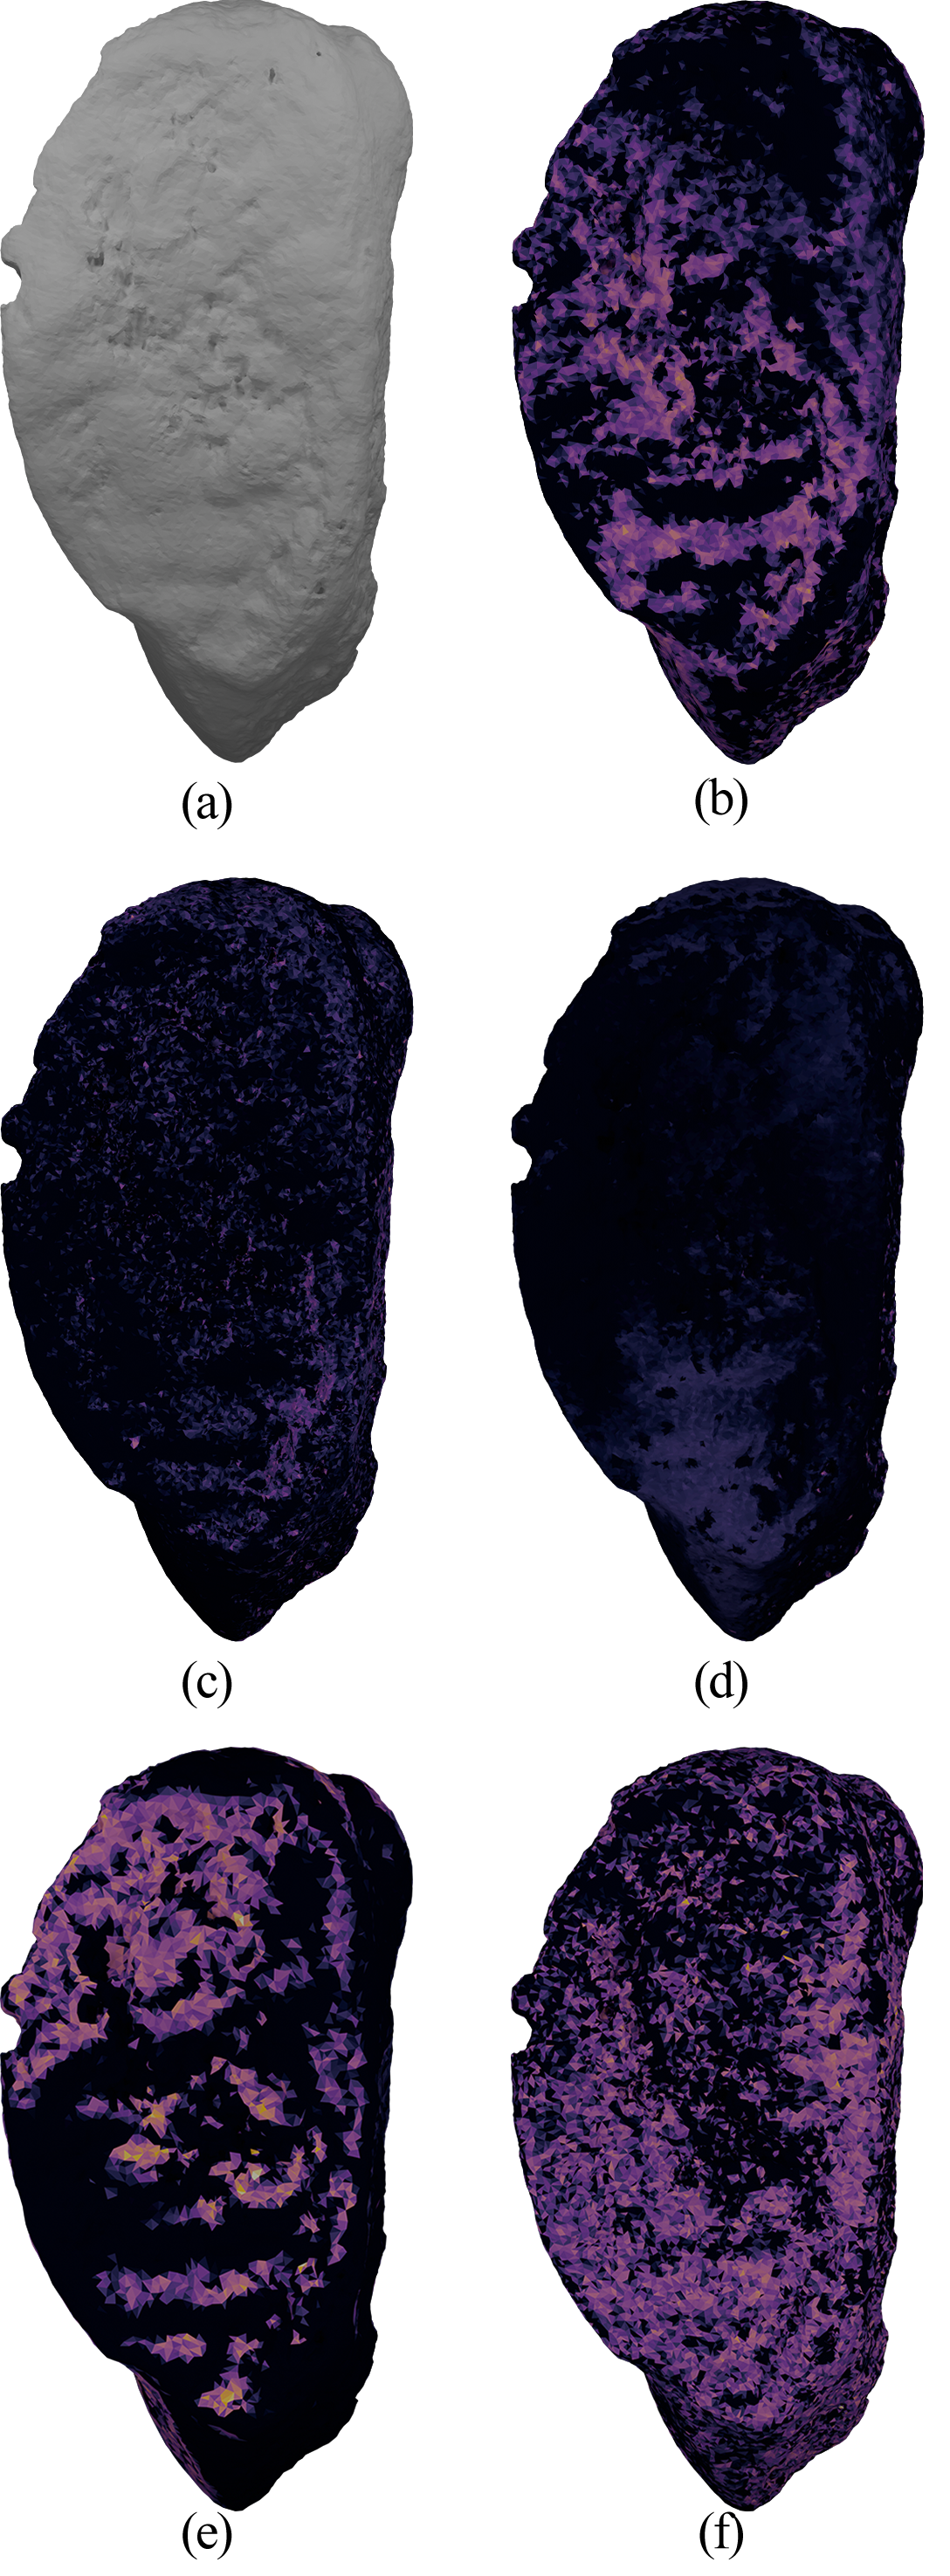
\includegraphics[width=0.5\linewidth]{figures/5_experiments/grad-cam-53-example.png}
    \caption[Ejemplo de mapas de activación de Grad-CAM correspondientes a distintas características para una misma muestra]{Ejemplo de los diferentes mapas de activación de Grad-CAM correspondientes a distintas características para una misma muestra. Los colores más cálidos indican una mayor activación. En (a) se muestra la malla original vista de frente. En este caso se visualizan las características AF (b), DM (c), IP (d), USE (e) y VM (f). Obsérvese cómo cada una se enfoca en regiones diferentes de la malla: algunas con activaciones bien definidas, como (b) y (e); otras con activaciones más dispersas o escasas, como (c) y (d); y (f), con activación en una gran parte de la superficie.}
    \label{fig5:grad_cam__diff_chars}
\end{figure}

\begin{figure}[p]
    \centering
    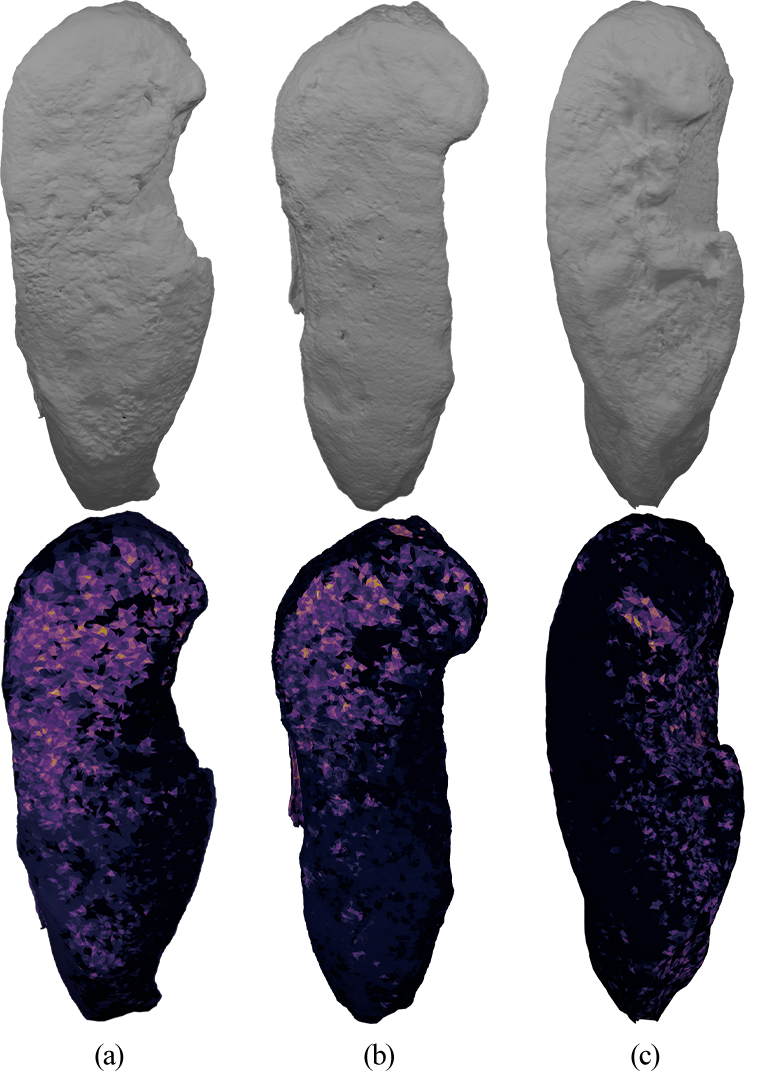
\includegraphics[width=\linewidth]{figures/5_experiments/grad-cam-BN-samples.png}
    \caption[Característica BN: Ejemplo de mapas de activación Grad-CAM]{Característica BN: Ejemplo de mapas de activación Grad-CAM. Se muestran tres mallas diferentes. En la parte superior se presentan las mallas originales, vistas de frente. En la parte inferior, las mismas mallas están coloreadas según la activación de Grad-CAM: los colores más cálidos indican una mayor activación. Se observa que el modelo se enfoca principalmente en la parte superior de la sínfisis del pubis. El modelo ha clasificado correctamente las mallas (a) y (b) como pertenecientes a la clase 0 (\say{ausente}), y la malla (c) a la clase 1 (\say{presente}).}
    \label{fig5:grad_cam__BN_samples}
\end{figure}

\begin{figure}[htbp]
    \centering
    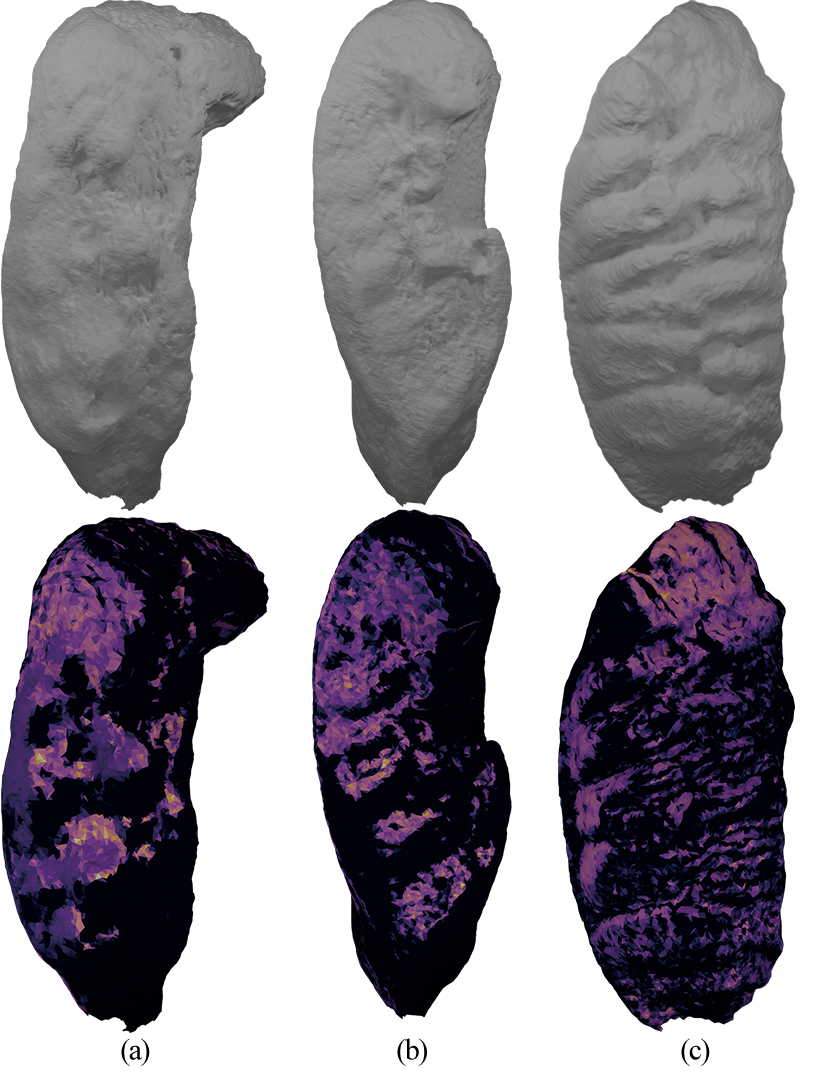
\includegraphics[width=\linewidth]{figures/5_experiments/grad-cam-USE-samples.png}
    \caption[Característica USE: Ejemplo de mapas de activación Grad-CAM]{Característica USE: Ejemplo de mapas de activación Grad-CAM. Se muestran tres mallas diferentes. En la parte superior se presentan las mallas originales, vistas de frente. En la parte inferior, las mismas mallas están coloreadas según la activación de Grad-CAM: los colores más cálidos indican una mayor activación. Se observa que el modelo tiende a enfocarse en la parte superior izquierda del hueso, con activaciones adicionales en los laterales y en zonas planas de la superficie. El modelo ha clasificado correctamente las mallas (a) y (b) como pertenecientes a la clase 1 (\say{definida}) y la malla (c) como 0 (\say{no definida}).}
    \label{fig5:grad_cam__USE_samples}
\end{figure}

\begin{figure}[htbp]
    \centering
    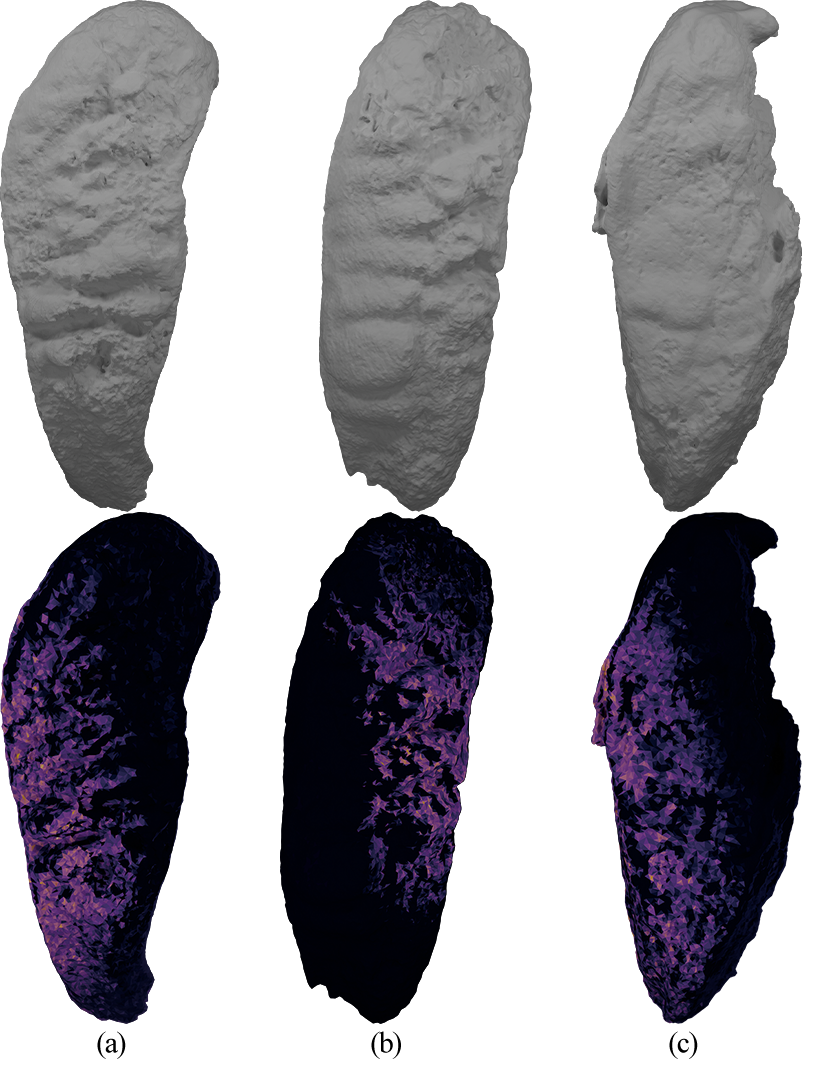
\includegraphics[width=\linewidth]{figures/5_experiments/grad-cam-DP-samples.png}
    \caption[Característica DP: Ejemplo de mapas de activación Grad-CAM]{Característica DP: Ejemplo de mapas de activación Grad-CAM. Se muestran tres mallas diferentes. En la parte superior se presentan las mallas originales, vistas de frente. En la parte inferior, las mismas mallas están coloreadas según la activación de Grad-CAM por triángulo: los colores más cálidos indican mayor activación. Se observa que el modelo se enfoca únicamente en un lateral del hueso. El modelo ha clasificado correctamente las mallas (a) y (c) como pertenecientes a la clase 0 (\say{ausente}), y la malla (b) como 1 (\say{presente}).}
    \label{fig5:grad_cam__DP_samples}
\end{figure}